% !TEX root = ../sommaire.tex

\chapter{Méthodologie et pipeline de traitement}

Ce chapitre décrit en détail la méthodologie proposée pour l'analyse automatisée d'organoïdes 3D via Graph Neural Networks. Nous présentons le pipeline complet depuis l'acquisition d'images jusqu'à la prédiction de phénotypes, en justifiant les choix effectués à chaque étape.

\section{Architecture générale du pipeline}

\subsection{Vue d'ensemble}

Notre pipeline transforme des images 3D brutes d'organoïdes en prédictions de phénotypes via une séquence d'étapes automatisées. Le flux de données est le suivant :

\begin{enumerate}
    \item \textbf{Input} : Image 3D confocale ($\sim$2 Go, 2048×2048×200 voxels)
    \item \textbf{Prétraitement} : Normalisation, débruitage, correction → Image nettoyée
    \item \textbf{Segmentation} : Faster Cellpose → Masques de segmentation (labels par cellule)
    \item \textbf{Extraction features} : Calcul des propriétés morphologiques → Table de features cellulaires
    \item \textbf{Clustering spatial} : DBSCAN → Séparation des organoïdes individuels
    \item \textbf{Construction graphes} : $\epsilon$-K-NN → Graphes géométriques ($\sim$10 Mo)
    \item \textbf{Classification GNN} : GNN → Prédiction du phénotype
    \item \textbf{Output} : Labels prédits
\end{enumerate}

Cette pipeline réduit la dimensionnalité de ~1000× (Go → Mo) tout en préservant l'information structurelle biologiquement pertinente.

\subsection{Choix de conception et compromis}

Chaque étape de notre pipeline résulte de choix méthodologiques motivés par des contraintes scientifiques, techniques et pratiques. Ces choix impliquent inévitablement des compromis que nous explicitons et justifions ici.

\subsubsection{Segmentation instance-based vs semantic}

Nous avons opté pour une segmentation d'instances, où chaque cellule individuelle reçoit un label unique, plutôt qu'une segmentation sémantique qui se contenterait de distinguer des catégories de cellules sans individualiser chaque objet. Ce choix est dicté par la nature même des graphes, qui requièrent des nœuds discrets et identifiables. L'identité individuelle de chaque cellule s'avère cruciale pour modéliser les relations spatiales et fonctionnelles entre cellules voisines — le cœur de l'approche par graphes. Une segmentation purement sémantique, bien que potentiellement plus rapide et robuste, ne fournirait pas la granularité nécessaire pour construire des graphes cellulaires exploitables, perdant l'information topologique fine qui constitue notre principale richesse analytique.

\subsubsection{Représentation graphe vs image brute}

La décision d'abstraire les organoïdes en graphes plutôt que de traiter directement les images volumétriques brutes constitue un choix architectural fondamental de cette thèse. Cette abstraction graphique apporte plusieurs avantages substantiels. D'abord, une compression spectaculaire : une réduction mémoire d'un facteur 1000 permet de stocker et manipuler des milliers d'échantillons sur du matériel standard. Ensuite, l'expressivité : le graphe capture explicitement les relations cellulaires (voisinage, distances, interactions) de manière structurée, là où une image ne présente qu'un champ d'intensités continues. Les invariances géométriques deviennent naturelles : rotation, translation et réflexion s'intègrent élégamment dans le formalisme graphique, particulièrement avec les architectures équivariantes. Enfin, l'interprétabilité : chaque nœud correspondant à une cellule identifiable, on peut remonter des prédictions du modèle aux cellules individuelles responsables, offrant une explicabilité biologiquement significative.

Ces avantages s'accompagnent toutefois de compromis qu'il convient de reconnaître. La qualité du graphe dépend intrinsèquement de la qualité de la segmentation en amont : toute erreur de segmentation se propage et contamine l'analyse ultérieure. L'abstraction graphique implique également une perte d'information sub-cellulaire — textures intra-cellulaires, gradients d'intensité locaux, organisation des organelles — qui pourrait porter des signatures phénotypiques subtiles. Enfin, la construction du graphe elle-même introduit des choix paramétriques (nombre de voisins K, rayon de connectivité) qui influencent les performances et nécessitent une exploration systématique. Malgré ces limitations, nous considérons que les bénéfices de l'approche graphique surpassent largement ses coûts, particulièrement dans notre contexte d'organoïdes 3D où la structure spatiale multi-échelle prime sur les détails texturaux fins.

\subsubsection{Graphes vs approches ensemblistes (DeepSets/PointNet)}

Une alternative intermédiaire entre images brutes (CNN) et graphes (GNN) consiste à représenter chaque organoïde comme un nuage de points — ensemble de positions cellulaires 3D avec features — traité par des architectures invariantes aux permutations comme DeepSets~\cite{Zaheer2017} ou PointNet~\cite{Qi2017}. Cette approche évite le coût mémoire des images volumétriques tout en garantissant l'invariance aux permutations (l'ordre de traitement des cellules n'affecte pas la prédiction).

\textbf{Limitations pour notre contexte :}

Malgré leur élégance théorique, ces approches présentent une limitation fondamentale : l'agrégation globale. Dans DeepSets, chaque élément est encodé indépendamment ($\phi(x_i)$) puis agrégé globalement ($\rho(\sum_i \phi(x_i))$). Aucune information sur les relations de voisinage spatial n'est explicitement capturée. Chaque cellule est traitée isolément avant l'agrégation finale.

Pour les organoïdes, cette limitation est critique. La structure spatiale locale — quelles cellules sont adjacentes, comment elles s'organisent en couches, où se forme le lumen — est biologiquement déterminante pour le phénotype. Par exemple :
\begin{itemize}
    \item La polarisation apico-basale dépend des contacts cellule-cellule (jonctions adhérentes)
    \item La formation du lumen requiert une coordination spatiale localisée
    \item La différenciation cellulaire est influencée par la signalisation paracrine des voisines directes
    \item Les patterns de prolifération exhibent une corrélation spatiale locale
\end{itemize}

Un modèle DeepSets/PointNet, en agrégeant globalement, rate ces patterns locaux critiques. En revanche, les GNNs propagent l'information itérativement via des voisinages structurés ($\sum_{j \in \mathcal{N}(i)} \psi(h_j)$), capturant explicitement les dépendances spatiales.

\textbf{PointNet++ et convergence vers les graphes :}

PointNet++~\cite{Qi2017b} adresse partiellement cette limitation via des agrégations locales hiérarchiques (set abstraction layers), se rapprochant conceptuellement des GNNs. Cependant, les voisinages sont définis par la distance euclidienne fixe à chaque couche, nécessitant de coûteuses recherches spatiales répétées. Les GNNs construisent le graphe une fois en amont puis réutilisent cette structure statique, offrant efficacité et contrôle précis de la topologie (K-NN adaptatif, seuils de distance).

\textbf{Choix justifié :}

Pour notre application, les GNNs offrent le meilleur compromis : compression mémoire (comme DeepSets), capture explicite de la structure spatiale locale (contrairement à DeepSets), efficacité computationnelle (graphe pré-construit), et équivariance géométrique formelle (EGNN).

\subsubsection{EGNN vs GNN standard}

Notre choix d'architectures équivariantes au groupe euclidien E(3), notamment EGNN, plutôt que de GNN standards (GCN, GAT) mérite justification. Les organoïdes cultivés en suspension 3D n'ont aucune orientation absolue privilégiée : leur position et orientation dans le milieu de culture sont entièrement aléatoires, dictées par les conditions physiques locales lors de l'ensemencement. Cette absence d'orientation canonique rend l'équivariance géométrique non pas simplement utile, mais véritablement indispensable pour des performances robustes. Un modèle équivariant garantit par construction que la prédiction reste identique quelle que soit l'orientation de l'organoïde dans l'espace — une propriété qu'un GNN standard devrait apprendre laborieusement via des augmentations de données exhaustives. Cette équivariance structurelle améliore également l'efficacité de l'utilisation des données : le modèle n'a pas besoin d'observer toutes les rotations possibles pour généraliser, réduisant les besoins en données annotées.

\subsection{Considérations pratiques}

\subsubsection{Temps d'exécution}

L'efficacité computationnelle du pipeline constitue un critère essentiel pour son adoption pratique. Sur une configuration standard (la nôtre : CPU Intel Core i7, GPU NVIDIA RTX 3080), le traitement d'un organoïde typique se décompose temporellement comme suit. Le prétraitement de l'image (normalisation, débruitage, corrections) s'exécute en moins d'une seconde sur CPU, tirant parti d'implémentations vectorisées efficaces. La segmentation cellulaire via Faster Cellpose requiert environ 20 minutes sur GPU selon la taille de l'organoïde — un temps considérablement réduit comparé aux 2.5 heures du Cellpose original. L'extraction des features morphologiques et intensimétriques opère rapidement en 1 à 2 secondes (CPU), suivie de la construction du graphe qui s'exécute en moins d'une seconde grâce aux structures de données spatiales efficaces (k-d trees). Enfin, l'inférence GNN elle-même ne prend qu'une fraction de seconde (moins de 0.1 sec) lorsque les graphes sont traités en batch sur GPU.

Le temps total s'établit ainsi à approximativement 20 minutes par organoïde, dominé par la segmentation cellulaire. L'avantage majeur du pipeline automatisé réside dans sa capacité à traiter des dizaines d'organoïdes en parallèle de manière non supervisée sur infrastructure GPU multi-cartes ou cluster de calcul. Cette parallélisation massive, combinée à l'automatisation complète (aucune intervention humaine requise) et à la reproductibilité parfaite des prédictions (élimination de la variabilité inter/intra-observateur), rend envisageable le criblage à haut débit de milliers d'organoïdes et ouvre des perspectives pour des études statistiquement puissantes à l'échelle de larges cohortes.

\subsubsection{Scalabilité}

L'architecture du pipeline a été conçue pour une parallélisation naturelle et efficace. Chaque organoïde constituant une unité de traitement indépendante, le pipeline peut traiter simultanément de multiples échantillons sans aucune dépendance ou communication inter-processus. Le batching de graphes pour l'inférence GNN exploite pleinement le parallélisme massif des GPUs modernes via le formalisme de graphes disjoints de PyTorch Geometric. Le déploiement sur clusters de calcul devient ainsi trivial : la charge de travail se distribue simplement entre nœuds de calcul sans nécessiter d'orchestration complexe.

Concrètement, pour traiter 1000 organoïdes, un workflow séquentiel sur une seule GPU nécessiterait approximativement 330 heures (environ 14 jours). Avec un déploiement parallèle sur 20 GPUs, ce temps se réduit à environ 17 heures, rendant praticable le retraitement complet d'un dataset dans des délais raisonnables. Cette scalabilité s'est révélée cruciale lors de nos campagnes d'ablation et d'optimisation d'hyperparamètres, où des centaines de configurations devaient être évaluées sur l'ensemble du dataset.

\section{Acquisition et prétraitement des images}

\subsection{Notre dataset collaboratif d'organoïdes de prostate}

\subsubsection{Contexte et partenariats}

Dans le cadre du projet ANR Morpheus et en collaboration avec l'IPMC (Nice) et l'équipe Metatox (Université Paris Cité), nous avons constitué un dataset d'organoïdes de prostate acquis entre mai 2023 et février 2025.

\begin{figure}[htbp]
    \centering
    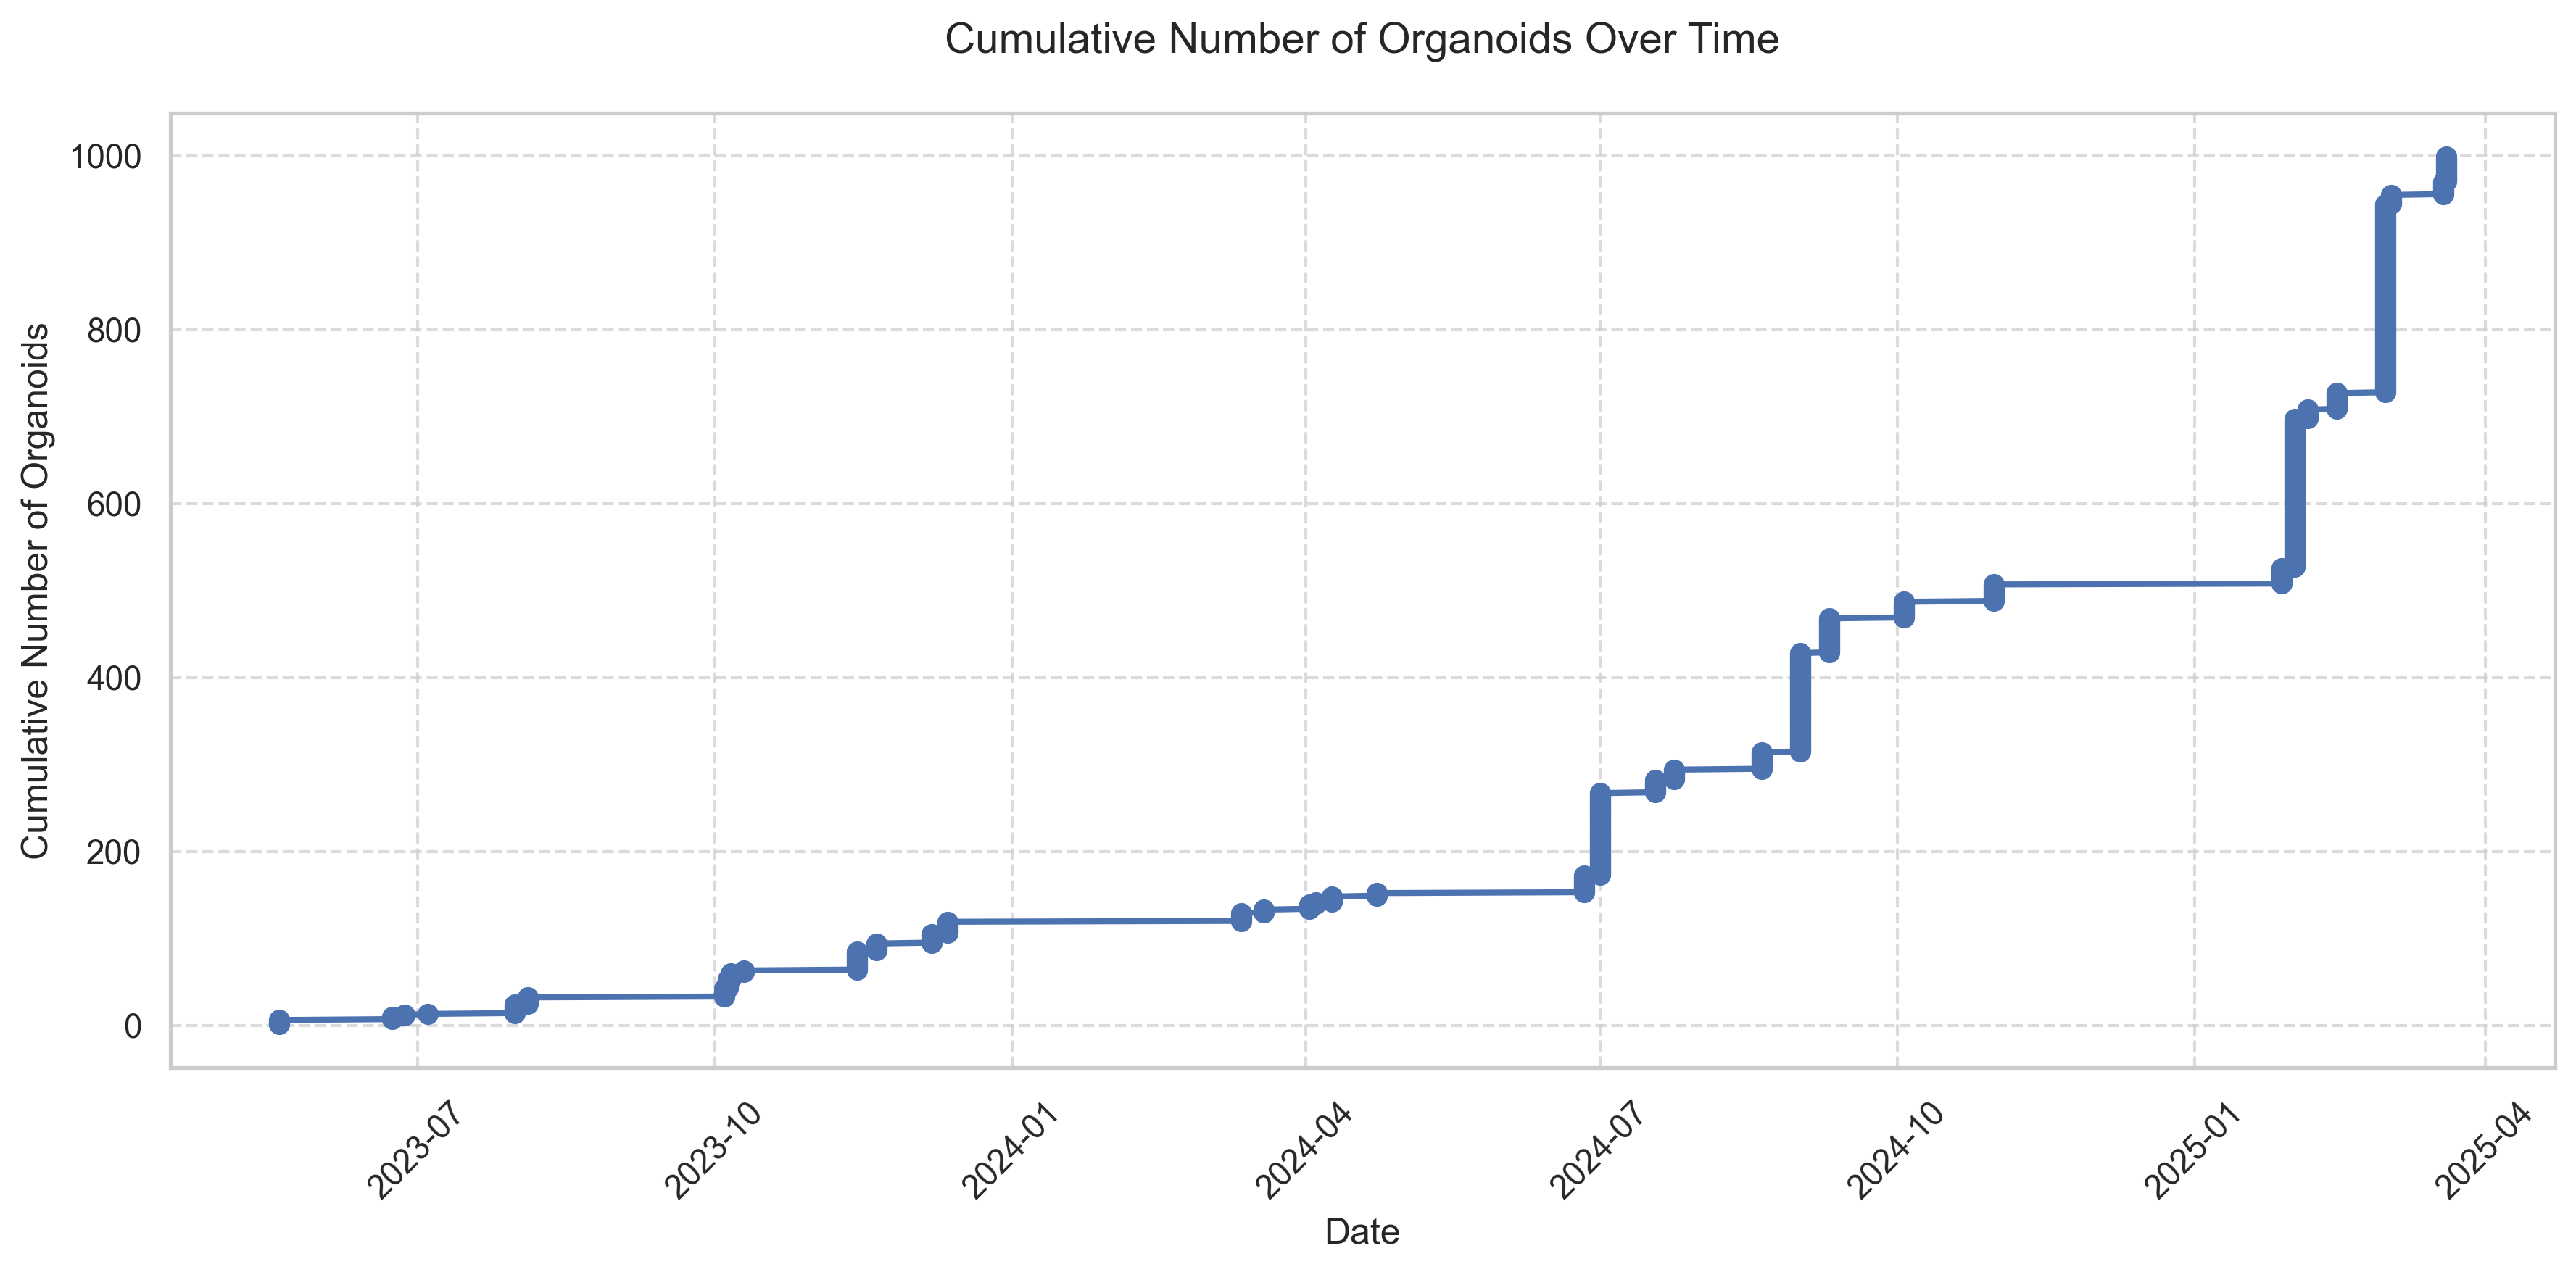
\includegraphics[width=0.75\textwidth]{../img/cumulative_organoids.png}
    \caption{Évolution cumulative du nombre d'échantillons acquis au cours du temps (mai 2023 - février 2025).}
    \label{fig:cumulative_organoids}
\end{figure}

\subsubsection{Caractéristiques du dataset}

Notre dataset constitue une ressource substantielle pour la recherche sur organoïdes, fruit de 22 mois de collecte continue entre mai 2023 et février 2025. Le volume total comprend 1311 échantillons imagés, dont l'analyse par clustering DBSCAN a permis d'extraire approximativement 2272 organoïdes individuels — reflétant la présence moyenne de 1.7 organoïdes par champ de vue. Pour cette étude, nous avons sélectionné 500 organoïdes bien différenciés présentant une concordance claire entre leur label batch et leur morphologie observée, les 1772 organoïdes restants (présentant une incohérence suspectée entre label et phénotype réel) étant réservés pour des approches non supervisées futures. Le pipeline génère environ 10310 fichiers au total, incluant les images TIF originales, les graphes au format JSON, et diverses visualisations PNG pour le contrôle qualité. En termes de stockage, les graphes compressés ne nécessitent qu'environ 200 Mo malgré leur richesse informationnelle, tandis que les images brutes volumétriques occupent approximativement 1To — illustrant une fois de plus la compression spectaculaire offerte par l'abstraction graphique.

\subsubsection{Phénotypes et distribution}

Deux phénotypes majeurs d'organoïdes de prostate dominent notre dataset et constituent le focus de notre étude, reflétant les architectures morphologiques les plus fréquemment observées dans les cultures d'organoïdes prostatiques.

Le phénotype \textit{Cystique} (Cystic) représente le phénotype sain de référence avec 528 échantillons (40.3\%), correspondant à environ 817 organoïdes individuels. Ces organoïdes se distinguent par la formation de kystes ou cavités internes, créant une structure creuse bordée d'un épithélium polarisé — une architecture rappelant les structures glandulaires prostatiques natives et témoignant d'une différenciation cellulaire appropriée. Au niveau de la distribution cellulaire, ce phénotype présente une répartition spatiale régulière et homogène, avec un espacement inter-cellulaire relativement uniforme caractéristique d'un processus proche du Poisson homogène ou d'un clustering très modéré. Cette organisation spatiale ordonnée reflète une morphogenèse tissulaire normale.

Le phénotype \textit{Choux-fleurs} (Cauliflower-like) constitue la classe perturbée majoritaire avec 732 échantillons (approximativement 55.9\%), correspondant à environ 1404 organoïdes individuels. Ces structures présentent une morphologie caractéristique en "chou-fleur" avec une surface fortement irrégulière parsemée de bourgeons multiples, évoquant une prolifération active et désorganisée. Au niveau cellulaire, ce phénotype se caractérise par une agrégation spatiale marquée : les cellules forment des clusters locaux denses séparés par des régions de densité moindre, créant une hétérogénéité spatiale prononcée. Cette organisation désordonnée rappelle les processus de Matérn cluster avec un fort coefficient d'agrégation et témoigne d'une perturbation des mécanismes normaux de différenciation et d'organisation tissulaire.

Ces deux phénotypes représentent ensemble 96.2\% du dataset et constituent notre problème de classification binaire principal : distinction entre le phénotype sain (cystique) et le phénotype perturbé (choux-fleurs). Bien que d'autres phénotypes minoritaires (compact, kératinisé) soient occasionnellement observés, leur rareté et leur variabilité limitent leur exploitation pour l'entraînement de modèles robustes, et nous les avons exclus de l'étude présente pour nous concentrer sur cette distinction biologiquement pertinente et statistiquement bien posée.

\subsubsection{Tâches d'apprentissage}

Au-delà de la classification de phénotypes, notre pipeline adresse une seconde tâche complémentaire : la régression de la déformation morphologique.

\textbf{Classification binaire (tâche principale) :}
Distinction choux-fleurs vs cystiques sur les données réelles. Cette tâche de classification supervisée constitue l'objectif applicatif principal, avec des métriques d'évaluation incluant accuracy, F1-score, et matrices de confusion.

\textbf{Régression du coefficient de clustering (tâche auxiliaire) :}
Sur les données synthétiques, nous entraînons les modèles à prédire le coefficient de clustering global du graphe — une variable continue dans $[0, 1]$ caractérisant le degré d'agrégation spatiale. Ce coefficient, défini comme la moyenne des coefficients de clustering locaux $\bar{C} = \frac{1}{N}\sum_{i=1}^N C_i$ où $C_i$ mesure la densité de triangles autour du nœud $i$, quantifie la tendance des cellules voisines à former des triades fermées. Pour les organoïdes générés par processus de Poisson homogène, $\bar{C} \approx 0$ (répartition aléatoire), tandis que pour les processus de Matérn avec forte agrégation, $\bar{C} \rightarrow 1$ (clusters denses). Cette tâche de régression sert de pré-entraînement auto-supervisé : le modèle apprend à extraire des représentations géométriques fines des patterns spatiaux cellulaires, représentations qui se transfèrent ensuite efficacement à la classification de phénotypes réels. L'erreur quadratique moyenne (MSE) et le coefficient de détermination $R^2$ servent de métriques d'évaluation pour cette tâche.

\textbf{Régression de la déformation morphologique (données réelles) :}
Pour les organoïdes réels, nous annotons également un score de déformation continue capturant le degré d'irrégularité morphologique — une mesure quantitative de l'écart par rapport à une sphère idéale. Cette métrique varie continûment entre les extrêmes cystiques (déformation faible, score ~0) et choux-fleurs (déformation forte, score ~1). La régression de ce score offre une granularité supérieure à la classification binaire, permettant de capturer les phénotypes intermédiaires et de quantifier finement les variations morphologiques intra-classe. Cette tâche utilise également la MSE comme loss et le $R^2$ comme métrique d'évaluation.

Ces trois tâches (classification binaire, régression synthétique, régression réelle) partagent le même encodeur GNN mais utilisent des têtes de prédiction différentes, permettant un entraînement multi-tâches optionnel ou séquentiel selon la stratégie adoptée.

\subsubsection{Protocole d'acquisition standardisé}

\textbf{Conditions de culture :}
\begin{itemize}
    \item \textbf{Timing} : Analyse au 7ème jour de culture (J7)
    \item \textbf{Marquage} : Noyaux + marqueurs spécifiques selon phénotype
\end{itemize}

\textbf{Paramètres d'imagerie :}
\begin{itemize}
    \item \textbf{Magnifications} : 20× (organoïdes cystiques de grande taille) ou 40× (standard)
    \item \textbf{Format} : Images 8-bit TIFF
    \item \textbf{Résolution} : 2048×2048 pixels (XY), 100-300 slices (Z)
\end{itemize}

\subsubsection{Pipeline de traitement et fichiers générés}

Chaque échantillon est traité via un pipeline automatisé générant plusieurs fichiers :

\textbf{Fichiers de base (fixes)} :
\begin{itemize}
    \item \texttt{raw\_*.tif} : Image brute microscopique (peut contenir plusieurs organoïdes)
    \item \texttt{cropped\_mask\_*.tif} : Masque de segmentation (labels cellulaires)
    \item \texttt{pointcloud\_*.json} : Nuage de points 3D de toutes les cellules
    \item \texttt{fullyconnected\_*.json} : Graphe complet entre toutes les cellules
    \item \texttt{centroids\_*.png} : Visualisation des centroïdes
    \item \texttt{clusters\_*.png} : Visualisation du clustering DBSCAN
\end{itemize}

\textbf{Fichiers par organoïde (variables)} :
\begin{itemize}
    \item \texttt{graph\_N\_*.json} : Graphe de l'organoïde N (N = 1, 2, 3, ...)
    \item \texttt{graph\_N\_*.png} : Visualisation du graphe de l'organoïde N
\end{itemize}

Le nombre de fichiers varie selon le nombre d'organoïdes détectés par DBSCAN :
\begin{itemize}
    \item \textbf{Base fixe} : 6 fichiers
    \item \textbf{Par organoïde} : +2 fichiers
    \item \textbf{Exemple} : 4 organoïdes détectés → 6 + 4×2 = 14 fichiers totaux
\end{itemize}

\subsubsection{Convention de nommage}

\textbf{Format 2023 (standard)} :
\begin{verbatim}
YYYYMMDD_Noyau_org[N]
Exemple : 20230804_Noyau_org1
\end{verbatim}

\textbf{Format 2024 (étendu Paris)} :
\begin{verbatim}
YYYY_MM_DD_[LIEU]_Noyau_Org_[N]_[phenotype]_J7_[magnification]_8bit
Exemple : 2024_07_18_PARIS_Noyau_Org_11_compact_J7_40X_8bit
\end{verbatim}

\textbf{Format 2024-2025 (Nice)} :
\begin{verbatim}
YYYYMM_Nice_orga[N]_[index]
Exemple : 202502_Nice_orga0_1
\end{verbatim}

\subsubsection{Métadonnées JSON}

Chaque fichier JSON contient des métadonnées structurées :

\begin{verbatim}
{
  "nodes": [
    {
      "cell_id": 1,
      "x": 531.305,
      "y": 152.108,
      "z": 12.987,
      "volume": 41644
    },
    ...
  ],
  "edges": [...],
  "metadata": {
    "organoid_name": "20230804_Noyau_org1",
    "phenotype": "Cystique"
  }
}
\end{verbatim}

\textbf{Informations capturées :}
\begin{itemize}
    \item Coordonnées spatiales 3D de chaque cellule
    \item Volume cellulaire
    \item Identifiants uniques de chaque cellule
    \item Connectivité entre cellules voisines
    \item Phénotype annoté
\end{itemize}

\subsubsection{Statistiques de taille}

\textbf{Distribution du nombre de cellules par organoïde :}
\begin{itemize}
    \item \textbf{Minimum} : ~20 cellules (seuil DBSCAN, filtre débris)
    \item \textbf{Maximum} : ~5,000 cellules (exclusion agrégats aberrants)
    \item \textbf{Moyenne} : ~250 cellules/organoïde
    \item \textbf{Médiane} : ~180 cellules/organoïde
    \item \textbf{Distribution} : Log-normale (queue lourde vers grandes tailles)
\end{itemize}

\textbf{Nombre moyen d'organoïdes par échantillon :}
~1.7 organoïdes/échantillon (variation : 1-6, dépend de la densité de culture et du champ de vue)

\subsubsection{Usage pour l'entraînement}

\textbf{Splits train/val/test :}
Stratification par phénotype pour préserver les distributions (sur les 500 organoïdes sélectionnés) :
\begin{itemize}
    \item \textbf{Train} : 70\% (~350 organoïdes)
    \item \textbf{Validation} : 15\% (~75 organoïdes)
    \item \textbf{Test} : 15\% (~75 organoïdes)
\end{itemize}

\textbf{Équilibrage des classes :}

La sélection de ~250 organoïdes par classe assure un parfait équilibre, éliminant les problèmes de déséquilibre de classes et permettant un apprentissage sans biais. Cette stratégie simplifie l'entraînement et garantit des performances équitables sur les deux phénotypes.

Ce dataset, bien que modeste (~500 organoïdes) comparé aux standards du deep learning (ImageNet : 14M images), est substantiel pour le domaine des organoïdes. Nous pallions cette limitation via la génération de données synthétiques (Section 4.6) et le transfer learning.

\subsection{Normalisation d'intensité}

Les intensités brutes varient selon les conditions d'acquisition (puissance laser, gain PMT, efficacité de marquage). Une normalisation est cruciale pour la robustesse.

\subsubsection{Normalisation par percentiles}

Plutôt qu'une normalisation min-max sensible aux outliers :
\[
I_{\text{norm}} = \frac{I - P_1}{P_{99} - P_1}
\]

où $P_1$ et $P_{99}$ sont les 1er et 99e percentiles de l'intensité. Cette méthode est robuste aux pixels aberrants.

\subsubsection{Correction de fond}

Le fond non-uniforme (autofluorescence, lumière diffusée) est estimé par un filtrage morphologique puis soustrait : $I_{\text{corr}} = I - I_{\text{fond}}$.

\subsection{Débruitage}

\subsubsection{Sources de bruit}

\textbf{Bruit photonique} : Fluctuations quantiques de photons (Poisson)

\textbf{Bruit de lecture} : Électronique du détecteur (Gaussien)

\textbf{Bruit de fond} : Autofluorescence, lumière ambiante

\subsubsection{Filtrage médian 3D}

Le filtre médian remplace chaque voxel par la médiane de son voisinage 3D. Excellent pour réduire le bruit impulsionnel (salt-and-pepper) tout en préservant les arêtes.

\subsubsection{Filtrage gaussien}

Convolution avec noyau gaussien 3D :
\[
I_{\text{filt}}(\mathbf{x}) = \int I(\mathbf{y}) \mathcal{N}(\mathbf{y}; \mathbf{x}, \sigma^2 \mathbf{I}) d\mathbf{y}
\]

Efficace pour le bruit gaussien mais lisse également les structures fines. Compromis via le paramètre $\sigma$.

\subsubsection{Choix pour notre pipeline}

Nous appliquons séquentiellement :
\begin{enumerate}
    \item Filtre médian 3×3×3 pour le bruit impulsionnel
    \item Filtre gaussien léger ($\sigma = 0.5$ voxels) pour le bruit résiduel
\end{enumerate}

Ce compromis préserve les détails cellulaires tout en améliorant le rapport signal sur bruit.

\section{Segmentation cellulaire automatisée}

La segmentation cellulaire constitue une étape critique, transformant l'image brute en objets discrets (cellules) analysables individuellement.

\subsection{Revue et comparaison des méthodes}

Nous avons évalué systématiquement plusieurs méthodes de segmentation sur un sous-ensemble annoté manuellement de 50 organoïdes. Pour une revue complète des méthodes de segmentation cellulaire et leurs applications au diagnostic, voir~\cite{Nunes2024,Rayed2024,Wang2022Segmentation}.

\subsubsection{StarDist}

\textbf{Principe :}
Détecte les centroides cellulaires puis prédit des distances radiales dans 96 directions uniformément distribuées, définissant un polyèdre star-convexe~\cite{Schmidt2018}.

\textbf{Résultats sur 50 coupes annotées :}
\begin{itemize}
    \item Précision : 0.97
    \item Rappel : 0.75
    \item F1-score : 0.85
    \item Temps : 5 sec/coupe
\end{itemize}

\textbf{Analyse :}
StarDist se distingue par une excellente précision dans la détection des noyaux cellulaires, bien que son rappel soit plus limité. Cette méthode s’avère particulièrement efficace lorsque les noyaux présentent des formes convexes, mais elle rencontre des difficultés dès lors que les morphologies deviennent irrégulières ou très allongées, c’est-à-dire lorsque les objets à segmenter ne sont plus star-convexes. De plus, StarDist s’avère sensible à la densité cellulaire élevée, ce qui entraîne des problèmes lors du traitement d’images avec de nombreux chevauchements entre noyaux. Plusieurs études comparatives~\cite{Weigert2022,Kleinberg2022} confirment l’intérêt et la polyvalence de StarDist dans divers contextes d’imagerie biologique, tout en soulignant qu’il est généralement dépassé par Cellpose lorsqu’il s’agit de segmenter des noyaux présentant une grande variété de formes.

\subsubsection{Cellpose}

\textbf{Principe :}
Prédit un champ de gradients où chaque pixel "pointe" vers le centre de sa cellule. Le suivi de ces gradients (flow tracking) regroupe les pixels en instances~\cite{Stringer2021}.

\textbf{Architecture :}
\begin{itemize}
    \item Encoder-decoder (U-Net-like) avec ResNet backbone
    \item Deux branches de sortie : gradients X et Y (2D) ou X, Y, Z (3D)
    \item Perte : erreur quadratique sur gradients + classificateur cellule/fond
\end{itemize}

\textbf{Résultats sur 50 coupes annotées :}
\begin{itemize}
    \item Précision : 0.99
    \item Rappel : 0.96
    \item F1-score : 0.98
    \item Temps : 30 sec/coupe
\end{itemize}

\textbf{Analyse :}
Cellpose est l'état de l'art en précision pour la segmentation de noyaux et de cellules en 3D. Il est robuste aux variations de taille, forme, densité. Les modèles pré-entraînés généralisent bien. La possibilité de fine-tuning permet d'améliorer encore les performances. Principal inconvénient : temps de calcul élevé pour l'analyse de milliers d'organoïdes.

\subsection{Contributions méthodologiques : optimisation de la segmentation}

\subsubsection{Problématique : lenteur de Cellpose standard}

Cellpose~\cite{Stringer2021}, bien qu'état de l'art en précision (F1=0.98), présente une limitation majeure pour notre contexte :

\textbf{Temps de calcul prohibitif :}
\begin{itemize}
    \item \textbf{Par coupe} : 30 secondes (GPU)
    \item \textbf{Par organoïde} : 30 sec × 300 coupes ≈ 2.5 heures
    \item \textbf{Pour 1000 organoïdes} : \textbf{2,500 heures (104 jours)}
    \item \textbf{Pour le dataset complet (2272 organoïdes)} : \textbf{5,680 heures (237 jours)}
\end{itemize}

Même avec une parallélisation sur 10 GPUs, cela représente plus de 3 semaines de calcul continu.

\textbf{Nécessité d'optimisation :}
Pour rendre le pipeline praticable sur nos milliers d'organoïdes, nous avons développé deux approches complémentaires de segmentation rapide.

\subsubsection{Contribution 1 : Méthode géométrique par détection d'ellipses}

\textbf{Principe :}
Approche déterministe basée sur la modélisation de noyaux comme ellipses, s'inspirant des processus ponctuels marqués. Cette approche géométrique s'inscrit dans une tradition de détection par ellipses~\cite{Kirsten2023}, mais optimisée pour les organoïdes 3D.

\textbf{Algorithme (détection 2D) :}
\begin{enumerate}
    \item Prétraitement : Flou gaussien ($\sigma=2$) + Black-Hat (rayon 15 px)
    \item Détection maxima locaux
    \item Pour chaque maximum, tester banque de filtres elliptiques $\{\epsilon_i\}$ paramétrés par :
        \begin{itemize}
            \item Angle $\theta_i = i\pi / I$ avec $I$ = nombre d'orientations
            \item Petit axe $a_i = a_{\min} + i \times \text{step}$ (de 3 à 25 pixels, pas de 2)
            \item Rapport d'aspect $r_i \in \{1.0, 1.5, 2.0, 2.5, 3.0\}$
        \end{itemize}
    \item Calculer réponse de convolution $(K_i * I)(x, y)$ avec noyau :
        \[
        K_i(x, y) = \begin{cases}
            1/|\epsilon_i| & \text{si } (x, y) \in \epsilon_i \\
            -1/|\partial \epsilon_i| & \text{si } (x, y) \in \partial \epsilon_i
        \end{cases}
        \]
    \item Retenir ellipse maximisant la réponse normalisée $R_{i,j} = (K_i * I)(p_j) / |\epsilon_i|$
    \item Seuillage adaptatif (70\% de la réponse max)
    \item Gestion des chevauchements : réduction progressive de l'ellipse la plus faible
\end{enumerate}

\textbf{Algorithme (appariement 3D) :}
\begin{enumerate}
    \item Pour chaque ellipse $\epsilon_n$ de la couche $z$, chercher candidates dans couche $z+1$
    \item Distance combinée :
        \[
        d(n, m) = 0.6 \cdot \frac{\|(x_n, y_n) - (x_m, y_m)\|^2}{15^2} + 0.3 \cdot \frac{|a_n - a_m|}{5} + 0.1 \cdot \frac{|\theta_n - \theta_m|}{\pi/2}
        \]
    \item Sélectionner meilleure candidate (min distance) si $d < 0.7$
    \item Fusionner en objet 3D
\end{enumerate}

\textbf{Performances obtenues sur 50 coupes annotées :}
\begin{table}[h]
\centering
\caption{Performances de notre méthode géométrique par ellipses}
\begin{tabular}{lcccc}
\toprule
\textbf{Méthode} & \textbf{Précision} & \textbf{Rappel} & \textbf{F1} & \textbf{Temps (s/coupe)} \\
\midrule
Notre méthode (2D seul) & 0.83 & 0.77 & 0.80 & 2 \\
Notre méthode (après 3D) & 0.91 & 0.85 & 0.88 & 3 \\
\midrule
\multicolumn{5}{l}{\textit{Pour comparaison : état de l'art}} \\
StarDist & 0.97 & 0.75 & 0.85 & 5 \\
Cellpose & 0.99 & 0.96 & 0.98 & 30 \\
\bottomrule
\end{tabular}
\end{table}

\begin{figure}[htbp]
    \centering
    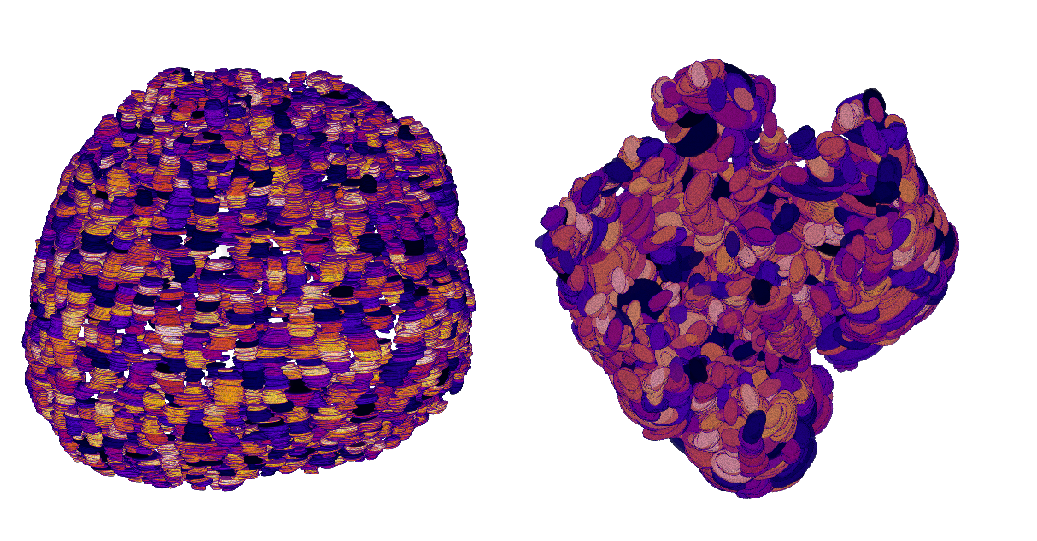
\includegraphics[width=0.9\textwidth]{../img/3Dreco.png}
    \caption{Visualisation 3D de la reconstruction par détection d'ellipses. Les ellipses détectées sur chaque coupe 2D sont empilées et appariées en 3D pour former les objets cellulaires complets. Chaque couleur représente une cellule individuelle identifiée par l'algorithme d'appariement 3D basé sur la distance combinée (position, taille, orientation).}
    \label{fig:3Dreco}
\end{figure}

\begin{figure}[htbp]
    \centering
    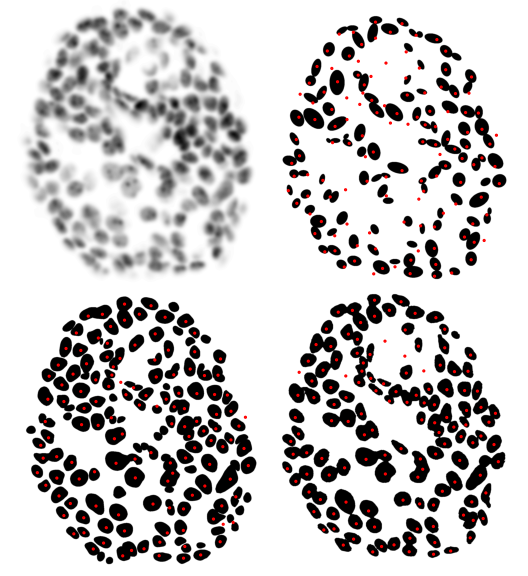
\includegraphics[width=0.95\textwidth]{../img/Comp.png}
    \caption{Comparaison qualitative des méthodes de segmentation sur une coupe représentative. De gauche à droite : image originale, segmentation par ellipses (notre méthode géométrique), StarDist, et Cellpose. Notre méthode géométrique par ellipses capture correctement la majorité des noyaux avec une précision acceptable (F1=0.88 après reconstruction 3D) tout en offrant une vitesse 10× supérieure à Cellpose.}
    \label{fig:comp}
\end{figure}

\textbf{Avantages :}
\begin{itemize}
    \item \textbf{Rapidité exceptionnelle} : 15× plus rapide que Cellpose
    \begin{itemize}
        \item 3 sec/coupe (avec reconstruction 3D) vs 30 sec/coupe (Cellpose)
        \item 250 heures vs 2,500 heures pour 1000 organoïdes
    \end{itemize}
    \item \textbf{Interprétabilité} : Paramètres géométriques explicites (axes, orientation, forme elliptique)
    \item \textbf{Sans entraînement} : Aucune annotation nécessaire, pas de phase d'apprentissage
    \item \textbf{Légèreté} : Fonctionne sur CPU standard, pas de GPU requis
    \item \textbf{Déterminisme} : Reproductibilité parfaite (pas de stochasticité)
\end{itemize}

\textbf{Limitations :}
\begin{itemize}
    \item Précision moindre : F1=0.88 vs 0.98 (Cellpose) après reconstruction 3D
    \item Hypothèse ellipsoïdale : cellules très irrégulières ou non-convexes mal gérées
    \item Cellules très petites (<5 pixels) ou très proches peuvent être manquées
    \item Nécessite images DAPI de bonne qualité (faible bruit, bon contraste)
\end{itemize}

\textbf{Cas d'usage :}
Cette méthode est adaptée pour le criblage primaire à très haut débit où le volume d'échantillons prime sur la précision absolue. Cependant, elle n'a pas été retenue pour notre pipeline final car la qualité de segmentation impacte directement la qualité des graphes et les performances des GNN en aval.

\subsubsection{Contribution 2 : Faster Cellpose via Knowledge Distillation}

\textbf{Collaboration :}
Cette optimisation a été développée en étroite collaboration avec Ivan Magistro Contenta (INRIA Sophia-Antipolis, équipe Morpheme), auteur principal de Faster Cellpose, que nous remercions chaleureusement pour son expertise et ses contributions essentielles à ce travail.

\textbf{Motivation :}
Obtenir la précision de Cellpose avec une vitesse acceptable pour nos milliers d'organoïdes réels et synthétiques.

\textbf{Approche : Knowledge Distillation}

Nous entraînons un modèle "étudiant" compact à partir du modèle Cellpose "enseignant" pré-entraîné.

\textbf{Architecture FastCellpose :}
L'architecture de FastCellpose repose sur une version simplifiée de Cellpose avec plusieurs optimisations structurelles. Le nombre de canaux est réduit à nbase = [16, 32, 64, 128] au lieu de [32, 64, 128, 256], permettant une réduction de 50\% du nombre de paramètres. L'upsampling est optimisé en utilisant des transposed convolutions plutôt que la combinaison bilinear + convolutions. Enfin, les skip connections sont allégées pour réduire la complexité globale du réseau.

\textbf{Entraînement par distillation :}
\begin{enumerate}
    \item \textbf{Teacher} : Cellpose cyto2 (pré-entraîné, frozen)
    \item \textbf{Student} : FastCellpose (entraînable)
    \item \textbf{Loss combinée} :
        \[
        \mathcal{L}_{\text{total}} = \alpha \mathcal{L}_{\text{hard}}(y_{\text{student}}, y_{\text{true}}) + \beta \mathcal{L}_{\text{soft}}(y_{\text{student}}, y_{\text{teacher}})
        \]
        où $\alpha = 0.3$, $\beta = 0.7$
    \item \textbf{Données} : 1000 organoïdes annotés (mixte manuel + prédictions enseignant)
    \item \textbf{Optimisation} : Adam, LR=1e-4, batch size=8, 100 époques
    \item \textbf{Validation} : 5-fold CV
\end{enumerate}

\textbf{Pruning additionnel :}
Après distillation, nous appliquons un pruning L1-unstructured sur 30\% des poids du réseau. Cette étape consiste à supprimer les connexions à faible magnitude, suivie d'un fine-tuning post-pruning sur 10 époques permettant une récupération des performances.

\textbf{Optimisations d'inférence :}
Plusieurs optimisations sont appliquées lors de l'inférence pour améliorer le débit de traitement. Le patch processing utilise des patchs de 256×256 pixels (au lieu de 224×224) avec un overlap de 64 pixels. La taille des batchs est augmentée à 16 (contre 8) pour un meilleur débit GPU. Enfin, le nombre d'itérations de flow tracking est réduit à 50 (contre 200 initialement), soit une réduction d'un facteur 4.

\textbf{Résultats Faster Cellpose :}
\begin{table}[h]
\centering
\caption{Performances de Faster Cellpose}
\begin{tabular}{lccccc}
\toprule
\textbf{Modèle} & \textbf{Params} & \textbf{Précision} & \textbf{F1} & \textbf{Temps (s/coupe)} & \textbf{Speedup} \\
\midrule
Cellpose original & 100\% & 0.99 & 0.98 & 30 & 1.0× \\
FastCellpose (distillation) & 50\% & 0.97 & 0.96 & 12 & 2.5× \\
+ Pruning 30\% & 35\% & 0.96 & 0.95 & 10 & 3.0× \\
+ Optimisations inférence & 35\% & 0.96 & 0.95 & 6 & 5.0× \\
\bottomrule
\end{tabular}
\end{table}

\textbf{Impact sur le temps total :}
L'impact de ces optimisations sur le temps de traitement est considérable. Pour 1000 organoïdes, le temps de calcul passe de 2,500 heures avec Cellpose original à 500 heures avec Faster Cellpose, soit un gain de 2,000 heures. Pour notre dataset complet, cela représente une réduction de 5,680 heures à 1,136 heures, soit un gain de 4,544 heures de temps de calcul.

\subsubsection{Choix final : Faster Cellpose}

\begin{figure}[htbp]
    \centering
    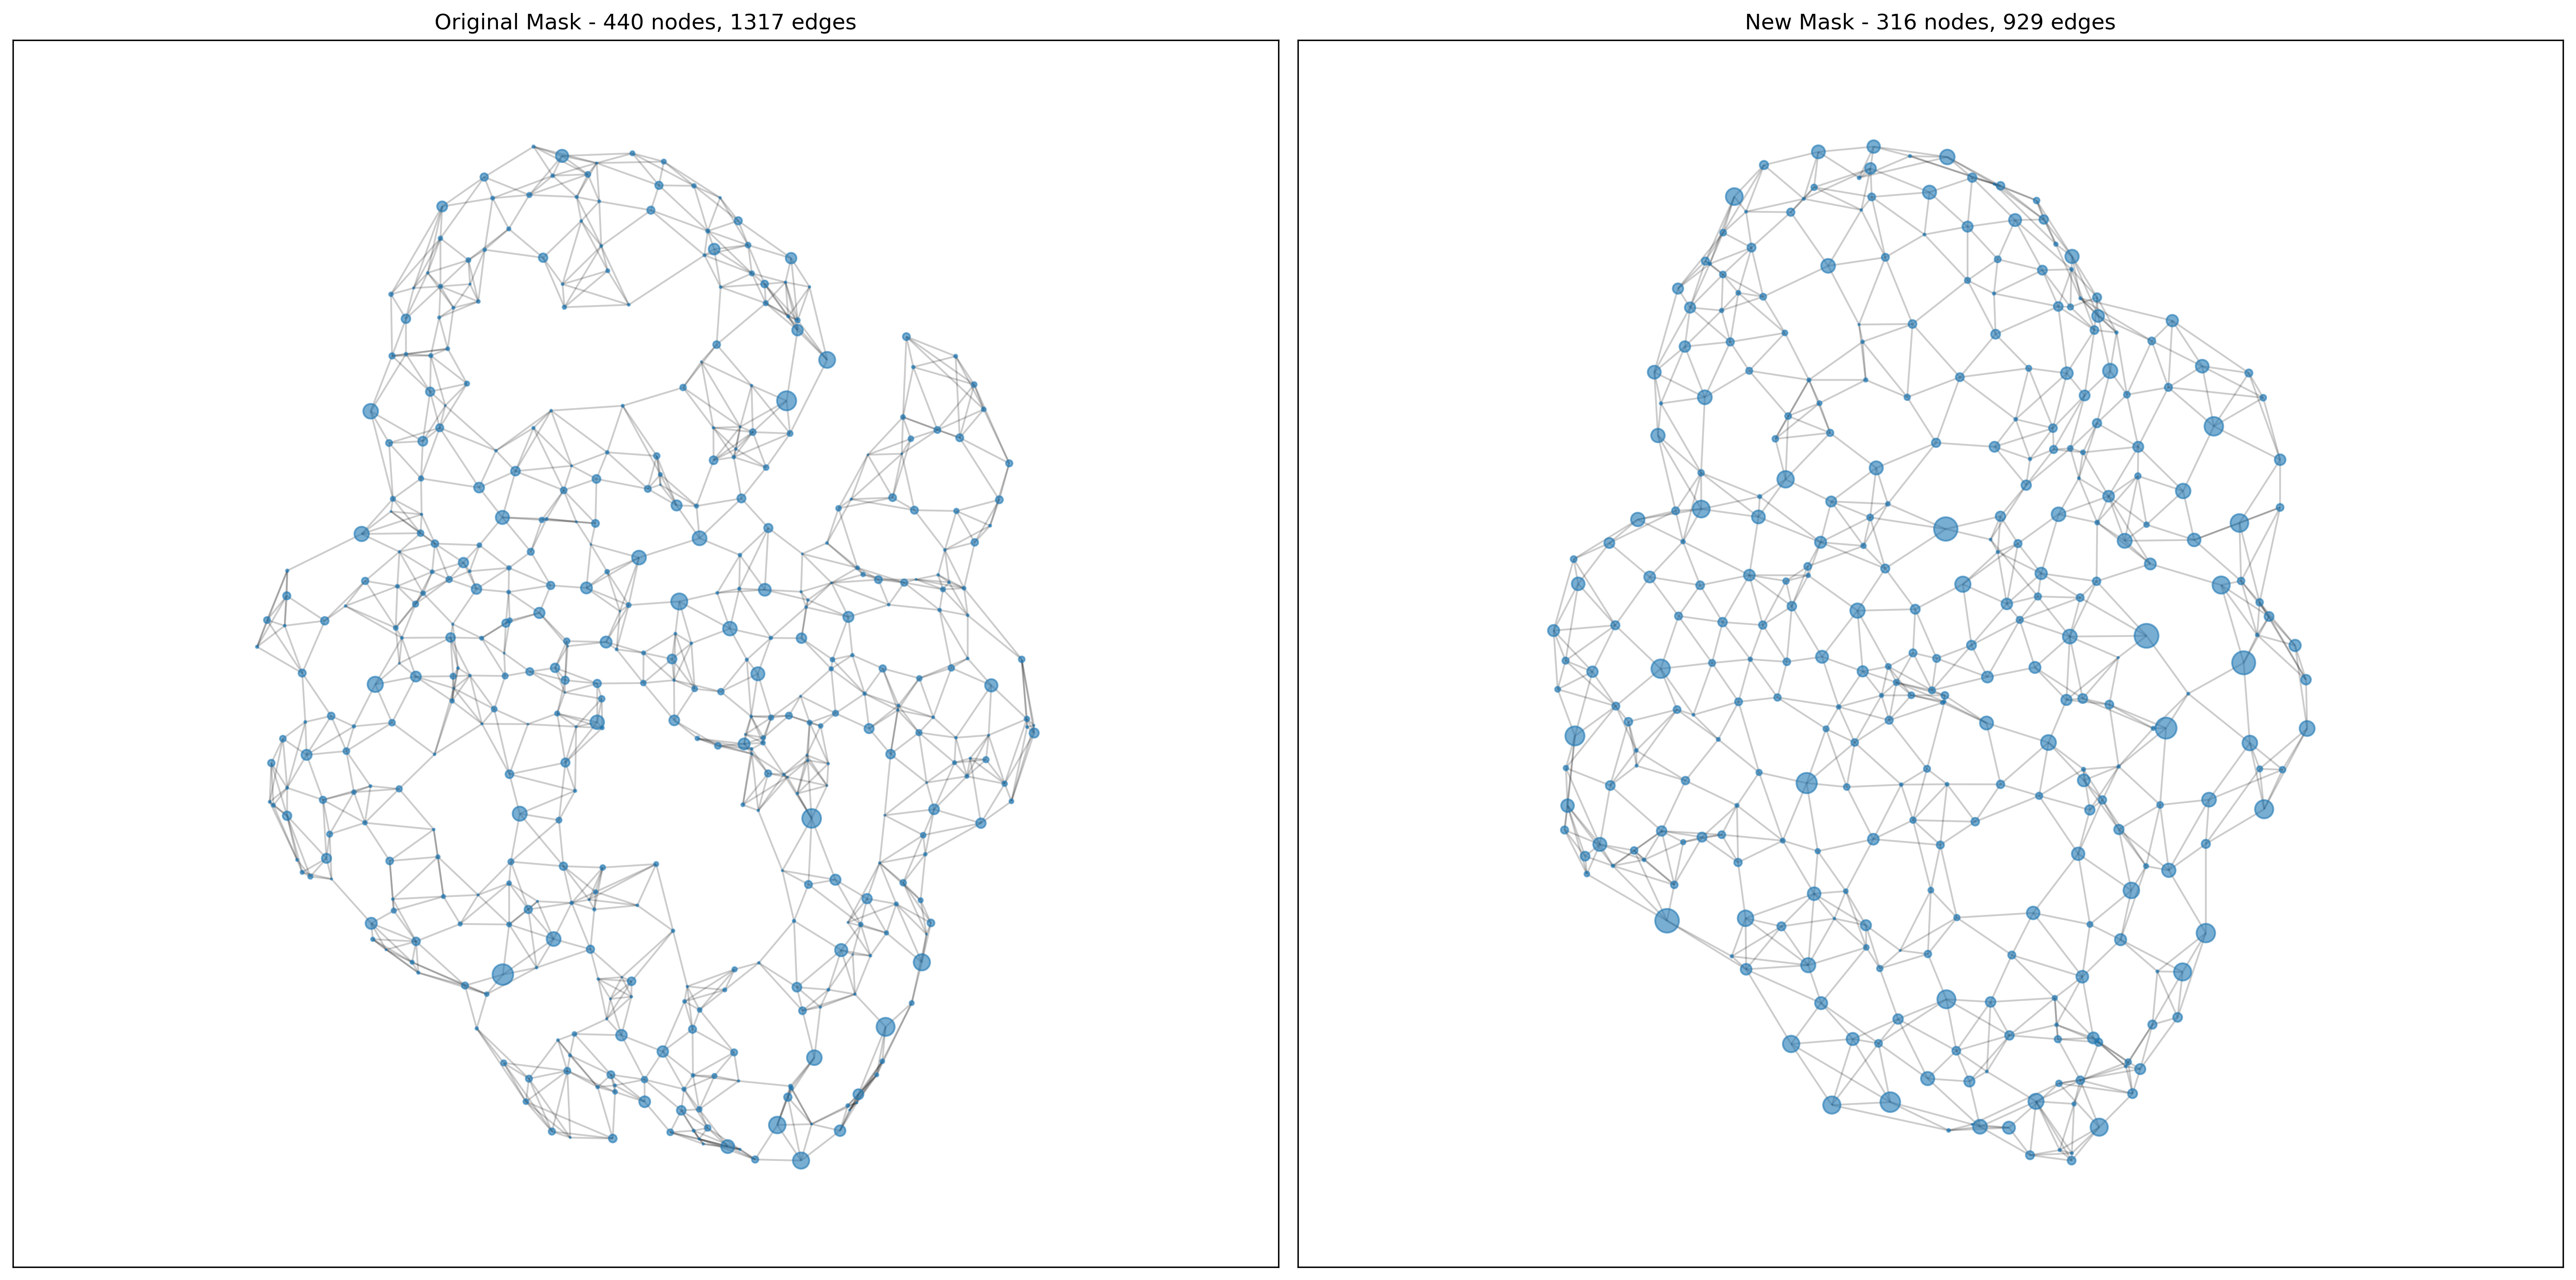
\includegraphics[width=0.85\textwidth]{../img/graph_comparison.png}
    \caption{Comparaison des graphes générés selon la méthode de segmentation utilisée. À gauche : graphe obtenu par la méthode géométrique par ellipses (3 sec/coupe, F1=0.88) montrant une topologie légèrement simplifiée avec quelques cellules manquées ou fusionnées. À droite : graphe obtenu par Faster Cellpose (6 sec/coupe, F1=0.95) présentant une structure plus dense et précise, capturant mieux les relations de voisinage cellulaire réelles. La qualité de segmentation impacte directement la topologie du graphe et donc les performances des GNN en aval, justifiant notre choix de Faster Cellpose comme méthode principale malgré un coût computationnel doublé.}
    \label{fig:graph_comparison}
\end{figure}

\textbf{Méthode retenue pour notre pipeline} : Faster Cellpose (distillation + pruning + optimisations)

\textbf{Justification :}
Le choix de Faster Cellpose comme méthode de segmentation pour notre pipeline se justifie par plusieurs facteurs convergents. En termes de précision, un F1-score de 0.95 constitue un niveau excellent, légèrement inférieur à Cellpose original mais largement suffisant pour nos besoins. La vitesse de traitement de 6 secondes par coupe, soit environ 30 minutes par organoïde, permet de traiter 1000 organoïdes en 500 heures (contre 2,500 heures pour Cellpose, soit un gain d'un facteur 5), et notre dataset complet de 2272 organoïdes en 1,136 heures (contre 5,680 heures pour Cellpose). Cette performance rend le traitement praticable avec 4 GPUs en environ 2 semaines, ou 10 GPUs en environ 5 jours. La qualité des graphes générés est préservée, les erreurs de segmentation restant minimales et n'impactant pas significativement l'apprentissage GNN en aval. En termes de ressources matérielles, Faster Cellpose fonctionne sur des GPU de 16 GB, contrairement aux 32 GB requis pour Cellpose original. Enfin, cette approche représente le compromis optimal entre précision et vitesse, surpassant la méthode géométrique (F1=0.88, 3 sec/coupe) en précision tout en restant suffisamment rapide pour notre application.

\textbf{Comparaison des 3 approches développées :}
\begin{table}[h]
\centering
\caption{Trade-off précision/vitesse de nos 3 approches de segmentation}
\begin{tabular}{lccccl}
\toprule
\textbf{Approche} & \textbf{F1} & \textbf{Temps/coupe} & \textbf{GPU} & \textbf{Total 1000 org.} & \textbf{Statut} \\
\midrule
Ellipses géométriques & 0.88 & 3 s & Non & 250h & Trop peu précis\\
\textbf{Faster Cellpose (utilisé)} & \textbf{0.95} & \textbf{6 s} & \textbf{Oui} & \textbf{500h} & \textbf{Pipeline principal} \\
Cellpose original & 0.98 & 30 s & Oui & 2500h & Trop lent \\
\bottomrule
\end{tabular}
\end{table}

\textbf{Note :} Les temps sont calculés pour 300 coupes par organoïde en moyenne.

\textbf{Paramètres Faster Cellpose utilisés :}
Les paramètres d'inférence de Faster Cellpose ont été optimisés pour notre application. Nous utilisons le modèle FastCellpose-nuclei (notre modèle distillé et pruné) avec un diamètre cellulaire de 17 pixels. Le traitement s'effectue par patchs de 256×256 pixels avec un overlap de 64 pixels, et un batch size d'inférence de 16. Le flow tracking est limité à 50 itérations avec un seuil de 0.4, tandis que le seuil de probabilité cellulaire (cellprob threshold) est fixé à 0.0. L'inférence utilise la précision mixte FP16 pour optimiser les performances GPU.

\textbf{Impact sur la thèse :}
Cette optimisation a permis de rendre praticable l'ensemble de notre pipeline, facilitant les itérations rapides lors du développement. Sans Faster Cellpose, cette thèse n'aurait pu être menée à bien dans les délais impartis.

\section{Extraction et séparation des organoïdes}

Une image de puits de culture contient typiquement plusieurs organoïdes à séparer.

\subsection{Conversion en nuages de points}

À partir des masques de segmentation, nous extrayons pour chaque cellule :
\begin{itemize}
    \item \textbf{Centroïde} : Position moyenne $(x_c, y_c, z_c) = \frac{1}{|C|}\sum_{(x,y,z) \in C} (x,y,z)$
    \item \textbf{Volume} : $V = |C| \cdot v_{\text{voxel}}$ où $v_{\text{voxel}}$ est le volume d'un voxel
\end{itemize}

Nous obtenons ainsi une table de features $(N_{\text{total}} \times 4)$ où $N_{\text{total}}$ est le nombre total de cellules dans l'image et 4 correspond aux coordonnées 3D et au volume.

\subsection{Clustering spatial par DBSCAN}

\textbf{Algorithme} : DBSCAN (Density-Based Spatial Clustering of Applications with Noise)

\textbf{Principe :}
Groupe les points denses en clusters, marque les points isolés comme du bruit.

DBSCAN a été choisi en raison de ses atouts spécifiques pour notre problématique. D'abord, cet algorithme n'exige pas de définir à l'avance le nombre de clusters à segmenter, contrairement à des méthodes comme K-means, ce qui le rend particulièrement adapté à des images dont le nombre d'organoïdes varie d'un échantillon à l'autre. De plus, DBSCAN se montre robuste face à la grande diversité de formes, capable de regrouper des clusters ayant des contours irréguliers — une caractéristique fréquente chez les organoïdes issus de cultures biologiques. Enfin, il gère efficacement le bruit inhérent aux données, comme les petits débris ou les artefacts issus d'erreurs de segmentation, en les étiquetant explicitement comme des points isolés plutôt qu’en les assignant à un groupe par défaut. Ces propriétés garantissent ainsi une séparation fiable et automatisée des différents organoïdes dans l'image.

\subsection{Filtrage}

Les clusters identifiés sont filtrés selon :
\begin{itemize}
    \item \textbf{Taille minimale} : ≥ 20 cellules (pour exclure les débris, fragments)
    \item \textbf{Taille maximale} : ≤ 5000 cellules (pour exclure les agrégats aberrants)
    \item \textbf{Centrage} : Rejet si trop proche des bords image (pour exclure les organoïdes coupés)
\end{itemize}

\subsubsection{Statistiques de séparation}

Sur un dataset de 50 images contenant 2-5 organoïdes par image, nous obtenons les résultats suivants :
\begin{itemize}
    \item Recall : 97\% (organoïdes manqués : très petits ou collés au bord)
    \item Précision : 99\% (faux positifs : agrégats de débris passant les filtres)
    \item Erreurs de fusion : < 1\% (deux organoïdes très proches confondus)
\end{itemize}

La séparation est donc très fiable, minimisant les erreurs propagées en aval.

\section{Construction de graphes géométriques}

Cette étape transforme chaque organoïde (nuage de points avec features) en graphe structuré.

\subsection{Définition des nœuds}

Chaque cellule segmentée devient un nœud $v_i$ du graphe, caractérisé par :

\subsubsection{Position 3D}

Coordonnées du centroïde : $\mathbf{x}_i = (x_i, y_i, z_i) \in \mathbb{R}^3$

\textbf{Normalization :}
Pour une invariance à la taille absolue de l'organoïde, les coordonnées sont centrées et normalisées :
\[
\mathbf{x}_i' = \frac{\mathbf{x}_i - \bar{\mathbf{x}}}{\text{std}(\mathbf{x})}
\]

où $\bar{\mathbf{x}}$ est le centroïde de l'organoïde.

\subsubsection{Features morphologiques}

Pour chaque cellule segmentée, nous extrayons un descripteurs morphologique essentiel :

\textbf{Volume cellulaire :}
\[
V_i = |C_i| \cdot v_{\text{voxel}}
\]
où $|C_i|$ est le nombre de voxels de la cellule $i$ et $v_{\text{voxel}}$ le volume d'un voxel.


\subsubsection{Vecteur de features final}

Le vecteur de features d'un nœud est constitué de quatre descripteurs géométriques et morphologiques :
\[
\mathbf{f}_i = [\text{position (3)}, \text{volume (1)}]^T \in \mathbb{R}^{4}
\]

comprenant les coordonnées 3D du centroïde $(x_i, y_i, z_i)$ et le volume cellulaire $V_i$.

\textbf{Normalisation :}
Le volume cellulaire est z-score normalisé sur le dataset d'entraînement :
\[
V'_i = \frac{V_i - \mu_V}{\sigma_V}
\]

pour assurer une contribution équilibrée et faciliter l'apprentissage.

\subsection{Stratégies de connectivité}

La construction des arêtes définit le voisinage et structure le graphe.

\subsubsection{K-Nearest Neighbors (K-NN)}

L'approche K-Nearest Neighbors consiste à connecter chaque nœud à ses $k$ plus proches voisins selon la distance euclidienne entre centroides. Cette méthode présente plusieurs avantages notables. Elle offre un degré contrôlé où chaque nœud possède exactement $k$ arêtes sortantes, permettant une structure prévisible. De plus, elle s'adapte naturellement à la densité locale, maintenant un nombre constant de connexions quelle que soit la concentration cellulaire. Enfin, elle garantit un graphe connexe dès lors que $k \geq 1$ et que l'organoïde est lui-même connexe.

Cependant, cette approche présente aussi des limitations. Le graphe K-NN est dirigé et asymétrique par nature : le fait que $i$ soit voisin de $j$ n'implique pas nécessairement que $j$ soit voisin de $i$. Cette asymétrie nécessite une symmétrisation explicite par union ou intersection des arêtes pour obtenir un graphe non-orienté.

Une étude de sensibilité détaillée (Section 5.3.3) a été menée sur différentes valeurs de $k \in \{5, 8, 10, 12, 15, 20\}$. Cette analyse a révélé que $k = 10$ constitue le choix optimal pour nos données, équilibrant connectivité locale et efficacité computationnelle.

\subsubsection{Rayon fixe (ε-radius)}

L'approche par rayon fixe connecte deux nœuds lorsque leur distance euclidienne est inférieure à un seuil $r$. Cette méthode offre plusieurs qualités intéressantes. Le graphe obtenu est non-orienté par construction, évitant le besoin de symmétrisation. L'interprétation géométrique est claire et intuitive, chaque cellule définissant une sphère d'influence de rayon $r$.

Néanmoins, cette méthode présente des inconvénients notables. Les degrés des nœuds deviennent très variables selon la densité locale, pouvant aller de 0 à plus de 50 connexions. De plus, la performance est sensible au choix du paramètre $r$, qui doit être ajusté selon les caractéristiques du dataset. Enfin, si $r$ est choisi trop petit, le graphe risque d'être déconnecté, fragmentant artificiellement l'organoïde en composantes isolées.

\subsubsection{Stratégie hybride retenue}

Pour notre pipeline, nous adoptons une approche hybride combinant les forces des méthodes K-NN et par rayon fixe. Le processus se déroule en trois étapes. D'abord, nous construisons un graphe K-NN initial avec $k = 10$ voisins par nœud, garantissant une connectivité contrôlée. Ensuite, nous symétrisons le graphe en ajoutant l'arête $(j,i)$ chaque fois qu'une arête $(i,j)$ existe, transformant le graphe dirigé en graphe non-orienté. Enfin, nous appliquons un filtre de distance en supprimant toutes les arêtes de longueur supérieure à $r_{\max}$, rejetant ainsi les connexions aberrantes entre cellules trop éloignées.

Cette stratégie hybride combine judicieusement les avantages du K-NN (degré contrôlé, adaptativité locale) et du rayon fixe (rejet des arêtes non-physiques, pertinence biologique), tout en atténuant leurs inconvénients respectifs.

\subsection{Features d'arêtes}

Chaque arête $(v_i, v_j)$ peut être enrichie de features optionnelles selon l'architecture GNN utilisée. La distance euclidienne $d_{ij} = \|\mathbf{x}_i - \mathbf{x}_j\|$ entre les centroides des deux cellules constitue la feature d'arête la plus fondamentale. Le vecteur directionnel unitaire $\mathbf{u}_{ij} = \frac{\mathbf{x}_j - \mathbf{x}_i}{\|\mathbf{x}_j - \mathbf{x}_i\|}$ encode l'orientation relative entre cellules voisines. Enfin, la similarité de features, calculée comme la distance L2 ou cosine entre $\mathbf{f}_i$ et $\mathbf{f}_j$, mesure la ressemblance morphologique entre cellules connectées.

Le choix des features d'arêtes dépend de l'architecture employée. Pour EGNN, seule la distance est utilisée afin de préserver l'équivariance géométrique E(3). Pour les GNN standards (GCN, GAT, GraphSAGE), toutes les features peuvent être exploitées sans contrainte d'équivariance.

\subsection{Analyse de sensibilité}

Une étude systématique détaillée au Chapitre 5 évalue l'impact des différents choix de construction sur les performances finales. Cette analyse explore plusieurs dimensions du design des graphes. Premièrement, nous comparons les stratégies de connectivité (K-NN pur, rayon fixe, triangulation de Delaunay, et notre approche hybride) pour identifier la plus performante. Deuxièmement, nous testons différentes valeurs du paramètre $k \in \{5, 8, 10, 12, 15, 20\}$ pour déterminer le nombre optimal de voisins. Troisièmement, nous explorons plusieurs rayons de coupure $r \in \{30, 50, 75, 100\}$ pour le filtrage des arêtes aberrantes. Quatrièmement, nous évaluons l'impact de la normalisation des coordonnées en comparant les performances avec et sans cette étape. Enfin, nous réalisons des études d'ablation sur les features morphologiques pour identifier celles qui contribuent le plus à la discrimination des phénotypes.

Cette analyse de sensibilité exhaustive guide nos choix finaux de conception et révèle les facteurs critiques influençant les performances, permettant d'optimiser chaque composante du pipeline de construction de graphes.

\section{Génération de données synthétiques}

La génération de données synthétiques constitue une contribution méthodologique majeure de cette thèse, adressant le problème critique de rareté d'annotations.

\subsection{Motivation et objectifs}

\subsubsection{Limites des approches classiques}

\textbf{Augmentation de données standard :}
Les techniques d'augmentation classiques~\cite{Shorten2019} (rotations, flips, élasticité, déformations, variations photométriques) génèrent des variations d'échantillons existants mais ne créent pas de nouvelles structures fondamentalement différentes. Elles ne permettent pas d'explorer l'espace complet des phénotypes possibles.

Les GANs et autres modèles génératifs d'images peuvent être proposés pour créer des images synthétiques d'organoïdes. Toutefois, cette approche soulève plusieurs limites majeures dans notre contexte. D'une part, l'entraînement de tels modèles requiert l'existence préalable de larges bases de données d'images annotées, ce qui ramène à la problématique initiale. D'autre part, la génération s'effectue au niveau du voxel, sans produire directement de segmentations ni de labels cellulaires exploitables pour des analyses morphologiques fines. En outre, le contrôle sur les labels phénotypiques demeure limité, rendant l'assignation de la classe générée souvent ambiguë voire arbitraire. Enfin, il demeure difficile de garantir et de valider le réalisme biologique des images produites par ces modèles, en l'absence de mesures quantitatives robustes pour comparer une image synthétique à la réalité expérimentale.

\textbf{Modèles génératifs de graphes classiques :}
Les modèles génératifs de graphes traditionnels, tels que le modèle d'Erdős-Rényi~\cite{Erdos1959}, le modèle de Barabási-Albert~\cite{Barabasi1999} ou le modèle de Watts-Strogatz~\cite{Watts1998}, offrent des mécanismes de génération de structures topologiques avec des propriétés statistiques contrôlables (degré moyen, coefficient de clustering, distribution des degrés). Cependant, ces modèles présentent plusieurs limitations critiques pour la génération d'organoïdes synthétiques. Premièrement, ils produisent uniquement des topologies abstraites sans information spatiale ni géométrique, alors que la distribution spatiale des cellules est fondamentale pour caractériser les phénotypes d'organoïdes. Deuxièmement, ces modèles ne capturent pas les contraintes biologiques inhérentes aux structures cellulaires (distances intercellulaires, répulsion stérique, organisation hiérarchique). Troisièmement, les graphes générés suivent des distributions statistiques génériques (loi de puissance, small-world) qui ne correspondent pas nécessairement aux motifs d'organisation observés dans les tissus biologiques. Enfin, l'absence de lien explicite entre les paramètres du modèle et les propriétés morphologiques des organoïdes rend difficile le contrôle précis des phénotypes générés et la validation biologique des structures produites.

\subsubsection{Notre approche : génération contrôlée et validable}

Nous proposons de générer des organoïdes synthétiques via un processus en deux étapes :
\begin{enumerate}
    \item \textbf{Distribution spatiale} : Processus ponctuel stochastique sur sphère → positions cellulaires
    \item \textbf{Géométrisation} : Construction du graphe via K-NN → structure topologique réaliste
\end{enumerate}

\textbf{Modélisation sphérique :}

Bien que les organoïdes de type chou-fleur ne présentent pas naturellement une morphologie parfaitement sphérique, nous adoptons une étape de projection sphérique qui s'avère essentielle pour établir un cadre de référence commun pour l'analyse comparative des phénotypes. Après normalisation des coordonnées, nous projetons les centres des noyaux cellulaires sur une sphère unité de rayon $R$. Cette transformation géométrique nous permet d'appliquer des processus ponctuels sphériques pour générer des distributions cellulaires synthétiques qui préservent les relations spatiales importantes entre cellules.

L'avantage principal de cette projection réside dans la normalisation des distances intercellulaires, facilitant ainsi la comparaison directe des motifs d'organisation cellulaire entre différents types d'organoïdes, indépendamment de leurs morphologies globales. Ce choix méthodologique constitue une hypothèse de travail fondamentale pour notre génération synthétique, permettant de nous concentrer sur la distribution spatiale des cellules plutôt que sur la forme externe de l'organoïde. Tous les points sont normalisés par le rayon de la sphère englobante pour simplifier les analyses et garantir la comparabilité.

\textit{Note méthodologique :} Cette représentation sphérique sert de base pour la validation statistique via les fonctions $K$ et $g$ (voir section suivante). Pour le dataset synthétique final destiné aux GNN, une transformation spatiale additionnelle étend ensuite les coordonnées au-delà de la sphère proportionnellement à la densité locale, simulant les protubérances en "chou-fleur" tout en préservant les aires cellulaires initiales (détails en section \ref{sec:dataset_final}).

\textbf{Avantages clés :}
\begin{itemize}
    \item \textbf{Contrôle fin} : Paramètres des processus ponctuels contrôlent directement les propriétés statistiques
    \item \textbf{Labels parfaits} : La classe (type de processus) est connue par construction
    \item \textbf{Segmentation parfaite} : Pas d'erreurs de segmentation dans synthétiques
    \item \textbf{Validation statistique rigoureuse} : Fonctions K, F, G comparables aux valeurs théoriques
    \item \textbf{Génération illimitée} : Pas de limite au nombre d'échantillons générables
    \item \textbf{Cadre géométrique unifié} : Normalisation sphérique permet application cohérente des statistiques spatiales
\end{itemize}

\subsection{Processus ponctuels implémentés}

Nous implémentons deux types de processus ponctuels formant un continuum de patterns spatiaux contrôlé par le coefficient de clustering.

\subsubsection{Processus de Poisson homogène (CSR)}

\textbf{Paramètre :} Intensité $\lambda$

\textbf{Interprétation :} Distribution aléatoire complète (Complete Spatial Randomness), référence de hasard sans structure spatiale particulière. Ce processus modélise des organoïdes où les cellules se répartissent sans interactions significatives, représentant un état de base neutre correspondant au phénotype cystique.

Les processus uniformes modélisent les organoïdes cystiques, où les cellules sont réparties aléatoirement à la périphérie d'une cavité centrale. Pour la sphère unité ($R=1$), la densité de probabilité est simplement :
\[
f(x,y,z) = \frac{3}{4\pi}, \quad \text{avec } x^2+y^2+z^2 \leq 1
\]

\textbf{Simulation :}
\begin{enumerate}
    \item $N \sim \text{Poisson}(4\pi \lambda)$
    \item Positions uniformes sur $\mathbb{S}^2$ générées par échantillonnage uniforme des coordonnées sphériques
\end{enumerate}

\subsubsection{Processus de Matérn cluster}

\textbf{Paramètres :} $\lambda_{\text{parent}}$, $\lambda_{\text{cluster}}$, $r$ (rayon de cluster)

\textbf{Interprétation :} Agrégation cellulaire contrôlée. Modélise des organoïdes avec niches locales de prolifération, formations de clusters correspondant à des zones de croissance active — un pattern caractéristique des organoïdes choux-fleurs réels. Ces structures présentent des amas cellulaires irréguliers résultant d'un processus parent-enfant hiérarchique.

\textbf{Simulation :}

Le processus de Matérn est généré par un mécanisme parent-enfant où les centres d'agrégats (parents) sont distribués uniformément sur la sphère. Puis, autour de chaque centre, des points (enfants) sont distribués selon une loi gaussienne tronquée de paramètre $\sigma$ (typiquement fixé à 0.15 dans notre étude comparative GRETSI~\cite{Martin2025GRETSI2}).

\begin{enumerate}
    \item Générer $N_c \sim \text{Poisson}(\lambda_{\text{parent}} \cdot 4\pi R^2)$ centres de clusters (points parents) uniformément sur $\mathbb{S}^2$
    \item Pour chaque centre, générer $N_k \sim \text{Poisson}(\lambda_{\text{cluster}} \cdot 4\pi r^2)$ points fils dans rayon $r$ (calotte sphérique)
    \item Les points enfants sont distribués autour du parent selon une loi gaussienne contrôlée par $\sigma$, puis reprojetés sur la sphère
\end{enumerate}

\textbf{Continuum de clustering :}
En faisant varier les paramètres $\lambda_{\text{parent}}$, $\lambda_{\text{cluster}}$ et $r$, nous générons un continuum de patterns allant du clustering faible (proche de Poisson) au clustering fort (agrégats marqués).

Cette paramétrisation permet de générer des organoïdes synthétiques couvrant le spectre des architectures spatiales observées dans les données réelles, du phénotype cystique relativement homogène au phénotype choux-fleur fortement agrégé.

\begin{figure}[htbp]
    \centering
    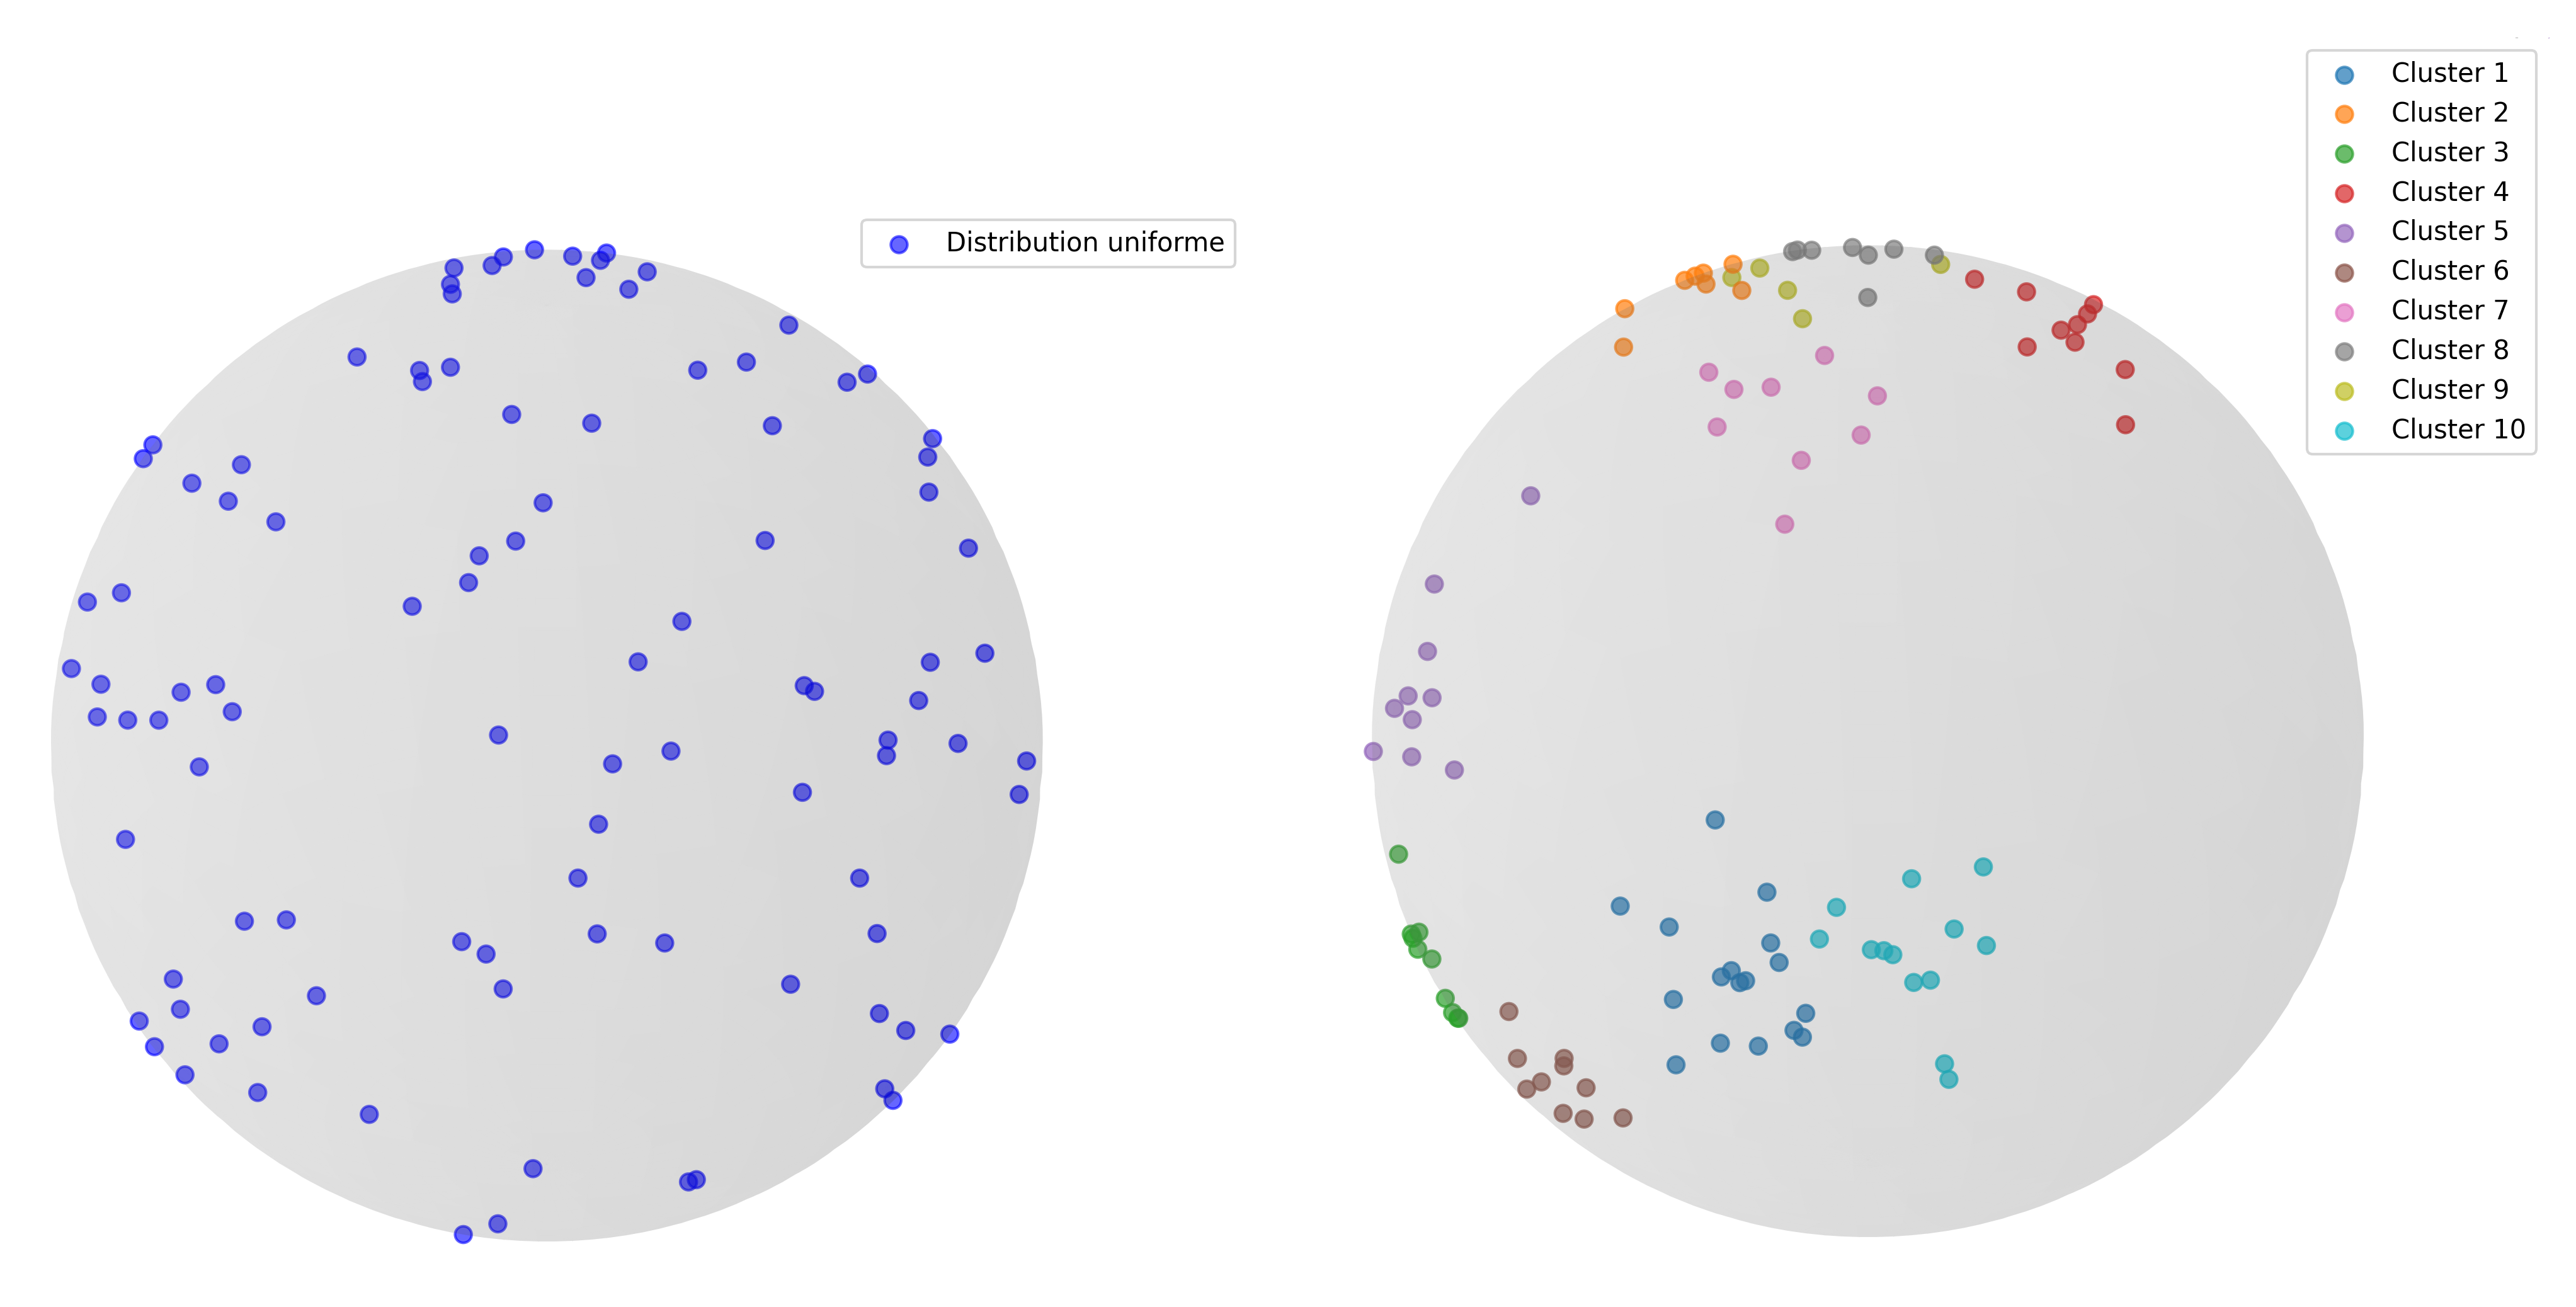
\includegraphics[width=0.85\textwidth]{../img/distrib2.png}
    \caption{Comparaison visuelle des deux processus ponctuels implémentés sur la sphère. À gauche : processus de Poisson homogène (CSR) générant une distribution uniforme et aléatoire des points représentant le phénotype cystique. À droite : processus de Matérn cluster produisant une distribution agrégée avec clusters locaux denses caractéristique du phénotype choux-fleur. Ces distributions sphériques servent de base pour la génération des organoïdes synthétiques et permettent l'application des statistiques spatiales sphériques pour validation.}
    \label{fig:distrib2}
\end{figure}

\subsection{Construction du graphe via tessellation de Voronoï sphérique}

À partir des positions cellulaires générées sur la sphère, nous construisons le graphe de connectivité en utilisant la tessellation de Voronoï sphérique, une structure naturelle capturant les relations de voisinage géométrique.

\subsubsection{Diagramme de Voronoï sphérique}

Pour les processus ponctuels sur la sphère $\mathbb{S}^2$, nous utilisons le diagramme de Voronoï sphérique qui partitionne la surface sphérique en régions basées sur la distance géodésique. La cellule de Voronoï sphérique du point $\mathbf{p}_i$ est définie comme :
\[
V_i^{\text{sph}} = \{\mathbf{x} \in \mathbb{S}^2 : d_{\text{geo}}(\mathbf{x}, \mathbf{p}_i) \leq d_{\text{geo}}(\mathbf{x}, \mathbf{p}_j) \, \forall j \neq i\}
\]
où $d_{\text{geo}}(\mathbf{x}, \mathbf{p}) = R \cdot \arccos(\mathbf{x} \cdot \mathbf{p})$ est la distance géodésique sur la sphère de rayon $R$ (pour des points normalisés).

Contrairement au diagramme de Voronoï euclidien 3D qui partitionne le volume $\mathbb{R}^3$ en polyèdres convexes, le Voronoï sphérique partitionne la surface de la sphère en régions sphériques polygonales, respectant la géométrie intrinsèque de la surface.

\subsubsection{Implémentation : scipy.spatial.SphericalVoronoi}

Nous utilisons l'implémentation de la classe SphericalVoronoi de la bibliothèque scipy qui calcule efficacement cette tessellation. L'algorithme :
\begin{enumerate}
    \item Prend en entrée les positions des points sur $\mathbb{S}^2$ (coordonnées cartésiennes 3D normalisées)
    \item Calcule le dual de l'enveloppe convexe 3D (triangulation de Delaunay) projeté sur la sphère
    \item Retourne les sommets et les régions de chaque cellule de Voronoï sphérique
\end{enumerate}

Chaque cellule de Voronoï sphérique est un polygone sphérique (délimité par des arcs de grands cercles), dont les sommets sont les points équidistants de trois sites voisins ou plus. Cette structure capture naturellement le voisinage géométrique : deux cellules partageant une arête correspondent à deux points spatialement adjacents.

\subsubsection{Construction du graphe}

La tessellation de Voronoï sphérique définit naturellement la connectivité du graphe :

\textbf{Règle de voisinage} : Deux nœuds $i$ et $j$ sont connectés par une arête si et seulement si leurs cellules de Voronoï $V_i^{\text{sph}}$ et $V_j^{\text{sph}}$ partagent une arête (arc de grand cercle). Cette règle garantit que seuls les voisins géométriquement adjacents sont connectés.

\textbf{Propriétés du graphe résultant} :
\begin{itemize}
    \item Graphe planaire : peut être projeté sur la sphère sans croisement d'arêtes
    \item Degré variable : chaque nœud a typiquement 5-7 voisins (théorème d'Euler pour graphes sphériques)
    \item Capture la géométrie locale : voisins proches dans l'espace euclidien 3D sont voisins dans le graphe
    \item Indépendant de l'orientation : invariant par rotations de la sphère
\end{itemize}

\subsubsection{Extraction de features}

Pour chaque cellule de Voronoï sphérique, nous calculons des propriétés géométriques servant de features pour les nœuds du graphe :

\textbf{Aire de la cellule} : Calculée comme l'aire du polygone sphérique, elle équivaut à l'excès sphérique :
\[
A_i = \left(\sum_{\text{angles}} \theta_k - (n-2)\pi\right) R^2
\]
où $n$ est le nombre de sommets et $\theta_k$ les angles internes du polygone sphérique.

\textbf{Correspondance avec le volume réel :}
Pour les données synthétiques générées sur la sphère, l'aire de la cellule de Voronoï $A_i$ sert de proxy pour la feature "volume" $V_i$ utilisée dans les graphes réels. Cette correspondance conceptuelle est justifiée géométriquement : dans les données réelles 3D, le volume mesure l'étendue spatiale occupée par la cellule ; dans les données synthétiques sphériques 2D-manifold, l'aire de Voronoï mesure analogiquement cette étendue sur la surface. Cette équivalence fonctionnelle garantit la cohérence sémantique des features entre données réelles et synthétiques, permettant l'apprentissage unifié des GNN sur les deux modalités. Ainsi, le vecteur de features synthétique contient $[x, y, z, A_i]$ où $A_i$ joue le rôle de $V_i$ des données réelles.

\textbf{Nombre de voisins} : Le degré du nœud dans le graphe, reflet de la densité locale.

Cette cohérence dans l'extraction des features entre données synthétiques et réelles garantit la transférabilité des représentations apprises. Les mêmes métriques géométriques calculées sur les tessellations de Voronoï sphériques des données réelles et synthétiques permettent une comparaison directe et un apprentissage cohérent.

\subsubsection{Calcul du coefficient de clustering pour la régression}

Une fois le graphe construit par tessellation de Voronoï, nous calculons son coefficient de clustering global $\bar{C}$, qui sert de label pour la tâche de régression sur données synthétiques.

\textbf{Définition mathématique :}

Pour chaque nœud $i$, le coefficient de clustering local mesure la proportion de triangles réalisés parmi ceux possibles dans son voisinage :
\[
C_i = \frac{2|\{(v_j, v_k) : v_j, v_k \in \mathcal{N}(i), (v_j, v_k) \in E\}|}{d_i(d_i-1)}
\]
où $\mathcal{N}(i)$ est l'ensemble des voisins du nœud $i$, $d_i$ son degré, et le numérateur compte le nombre d'arêtes reliant les voisins entre eux (formant des triangles avec $i$).

Le coefficient de clustering global du graphe est la moyenne sur tous les nœuds :
\[
\bar{C} = \frac{1}{N}\sum_{i=1}^N C_i
\]

\textbf{Relation avec le continuum Poisson-Matérn :}

Ce coefficient quantifie la tendance des cellules voisines à former des groupes densément connectés, capturant ainsi le degré d'agrégation spatiale :

\begin{itemize}
    \item \textbf{Poisson homogène} : Les cellules sont distribuées aléatoirement sur la sphère. Les voisins d'une cellule ont peu de chance d'être eux-mêmes voisins $\Rightarrow$ $\bar{C} \approx 0.1$-$0.2$ (faible clustering)
    
    \item \textbf{Matérn cluster} : Les cellules forment des amas locaux. Les voisins d'une cellule appartiennent souvent au même cluster et sont donc connectés entre eux $\Rightarrow$ $\bar{C} \approx 0.7$-$0.9$ (fort clustering)
    
    \item \textbf{Continuum intermédiaire} : En variant les paramètres du processus de Matérn ($\lambda_{\text{parent}}$, $\lambda_{\text{cluster}}$, $r$), nous générons des patterns avec des degrés d'agrégation variables, produisant des valeurs de $\bar{C}$ couvrant uniformément l'intervalle $[0, 1]$
\end{itemize}

\textbf{Propriété clé :} Le coefficient de clustering $\bar{C}$ est calculé \textit{a posteriori} sur le graphe généré, après application du processus ponctuel et construction de la tessellation. Il capture implicitement les corrélations spatiales induites par les paramètres du processus, offrant ainsi une métrique univoque et continue du degré d'organisation spatiale, idéale pour une tâche de régression supervisée.

\subsection{Stratégies d'augmentation}

Au-delà de la génération de base via processus ponctuels, nous appliquons des transformations stochastiques additionnelles pour diversifier le dataset synthétique et améliorer sa représentativité de la variabilité biologique réelle.

\subsubsection{Simulation de bruit d'acquisition}

Pour évaluer la robustesse de nos modèles face aux imperfections expérimentales et préparer les GNN aux variations présentes dans les données réelles, nous appliquons deux types de bruit aux distributions synthétiques~\cite{Martin2025GRETSI2} :

\textbf{Bruit gaussien :}
Un bruit gaussien $\mathcal{N}(0, \sigma_g^2)$ est appliqué aux coordonnées de chaque point, simulant les incertitudes de localisation dues aux limitations optiques et aux erreurs de segmentation. Dans nos études de robustesse, nous faisons varier $\sigma_g$ de 0 à 0,8 par pas de 0,1, permettant d'évaluer la dégradation des performances sous bruit croissant. Ce type de bruit altère les positions cellulaires tout en préservant la structure globale de la distribution.

\textbf{Bruit poivre et sel :}
Ce bruit modifie la structure même de la distribution en ajoutant et supprimant aléatoirement des points, simulant les erreurs de détection cellulaire :
\begin{itemize}
    \item \textbf{Composante "sel"} : Ajout de points uniformément répartis sur la sphère (fausses détections, débris cellulaires)
    \item \textbf{Composante "poivre"} : Suppression aléatoire de points existants (cellules non détectées, segmentation incomplète)
\end{itemize}

L'intensité du bruit poivre et sel $\sigma_{ps}$ varie de 0 à 0,4 par pas de 0,05, où $\sigma_{ps}$ représente la proportion de points affectés (ajoutés ou supprimés). Ce type de bruit est particulièrement pertinent car il reproduit fidèlement les erreurs de segmentation observées dans les pipelines d'analyse réels.

\textbf{Contrainte sphérique :}
Il est important de noter que nous contraignons les points à rester sur la sphère après bruitage (par reprojection radiale), maintenant ainsi la cohérence géométrique nécessaire pour l'application des statistiques spatiales sphériques et garantissant que les graphes construits demeurent valides. Cette contrainte reflète également la réalité biologique où les cellules restent confinées à la périphérie de l'organoïde.

\subsubsection{Dataset synthétique final}
\label{sec:dataset_final}

Le dataset synthétique final comprend environ 100~000 organoïdes générés le long du continuum Poisson-Matérn, avec une densité d'échantillonnage plus importante aux extrêmes (Poisson pur, Matérn fortement clustérisé) et dans les régions intermédiaires correspondant aux phénotypes réels observés. Chaque organoïde contient en moyenne 250 cellules (plage de 50 à 500 cellules), calibrée sur les distributions réelles. Le dataset est partitionné stratégiquement : 70\% pour l'entraînement (70~000 organoïdes), 15\% pour la validation (15~000 organoïdes), et 15\% pour le test (15~000 organoïdes). L'ensemble ne nécessite qu'approximativement 10 Go de stockage (graphes au format JSON compressé), rendant sa manipulation aisée.

\textbf{Transformation spatiale pour les GNN :}
Une distinction méthodologique importante doit être soulignée concernant la représentation spatiale des données. Alors que les études comparatives avec les statistiques spatiales sphériques (Ripley's $K$, fonction $g$) nécessitent de maintenir les points strictement sur la surface sphérique (comme décrit précédemment), le dataset synthétique final destiné à l'entraînement des GNN subit une transformation spatiale additionnelle visant à mieux simuler la morphologie réelle des organoïdes de type "chou-fleur".

Concrètement, après génération initiale des positions cellulaires sur la sphère selon les processus ponctuels choisis, nous appliquons une extension radiale des coordonnées proportionnelle à la densité locale de voisinage. Pour chaque cellule $i$ de position initiale $\mathbf{p}_i$, la position finale devient :
\[
\mathbf{p}_i' = \mathbf{p}_i \cdot \left(1 + \alpha \cdot \frac{|\mathcal{N}_r(i)|}{|\mathcal{N}_r^{\text{ref}}|}\right)
\]
où $\mathcal{N}_r(i)$ désigne le voisinage de rayon $r$ autour de $i$, $|\mathcal{N}_r^{\text{ref}}|$ est une taille de voisinage de référence (médiane ou moyenne globale), et $\alpha$ contrôle l'ampleur de l'extension (typiquement $\alpha \in [0.2, 0.5]$). Cette transformation étend les points au-delà de la sphère initiale dans les régions de forte densité locale (clusters), reproduisant ainsi les protubérances observées dans les organoïdes réels.

\textbf{Principe et conservation :}
Cruciale, cette transformation préserve l'aire associée initiale à chaque cellule (telle que déterminée par le diagramme de Voronoï ou les méthodes de segmentation), ne modifiant que les coordonnées spatiales. Ainsi, les features géométriques liées aux aires cellulaires demeurent cohérentes avec la distribution initiale sur la sphère, tandis que la structure spatiale 3D reflète mieux la réalité morphologique des organoïdes cultivés. Cette dualité permet d'exploiter la rigueur théorique des statistiques spatiales sphériques pour la validation tout en entraînant les GNN sur des géométries plus réalistes.

\begin{figure}[htbp]
    \centering
    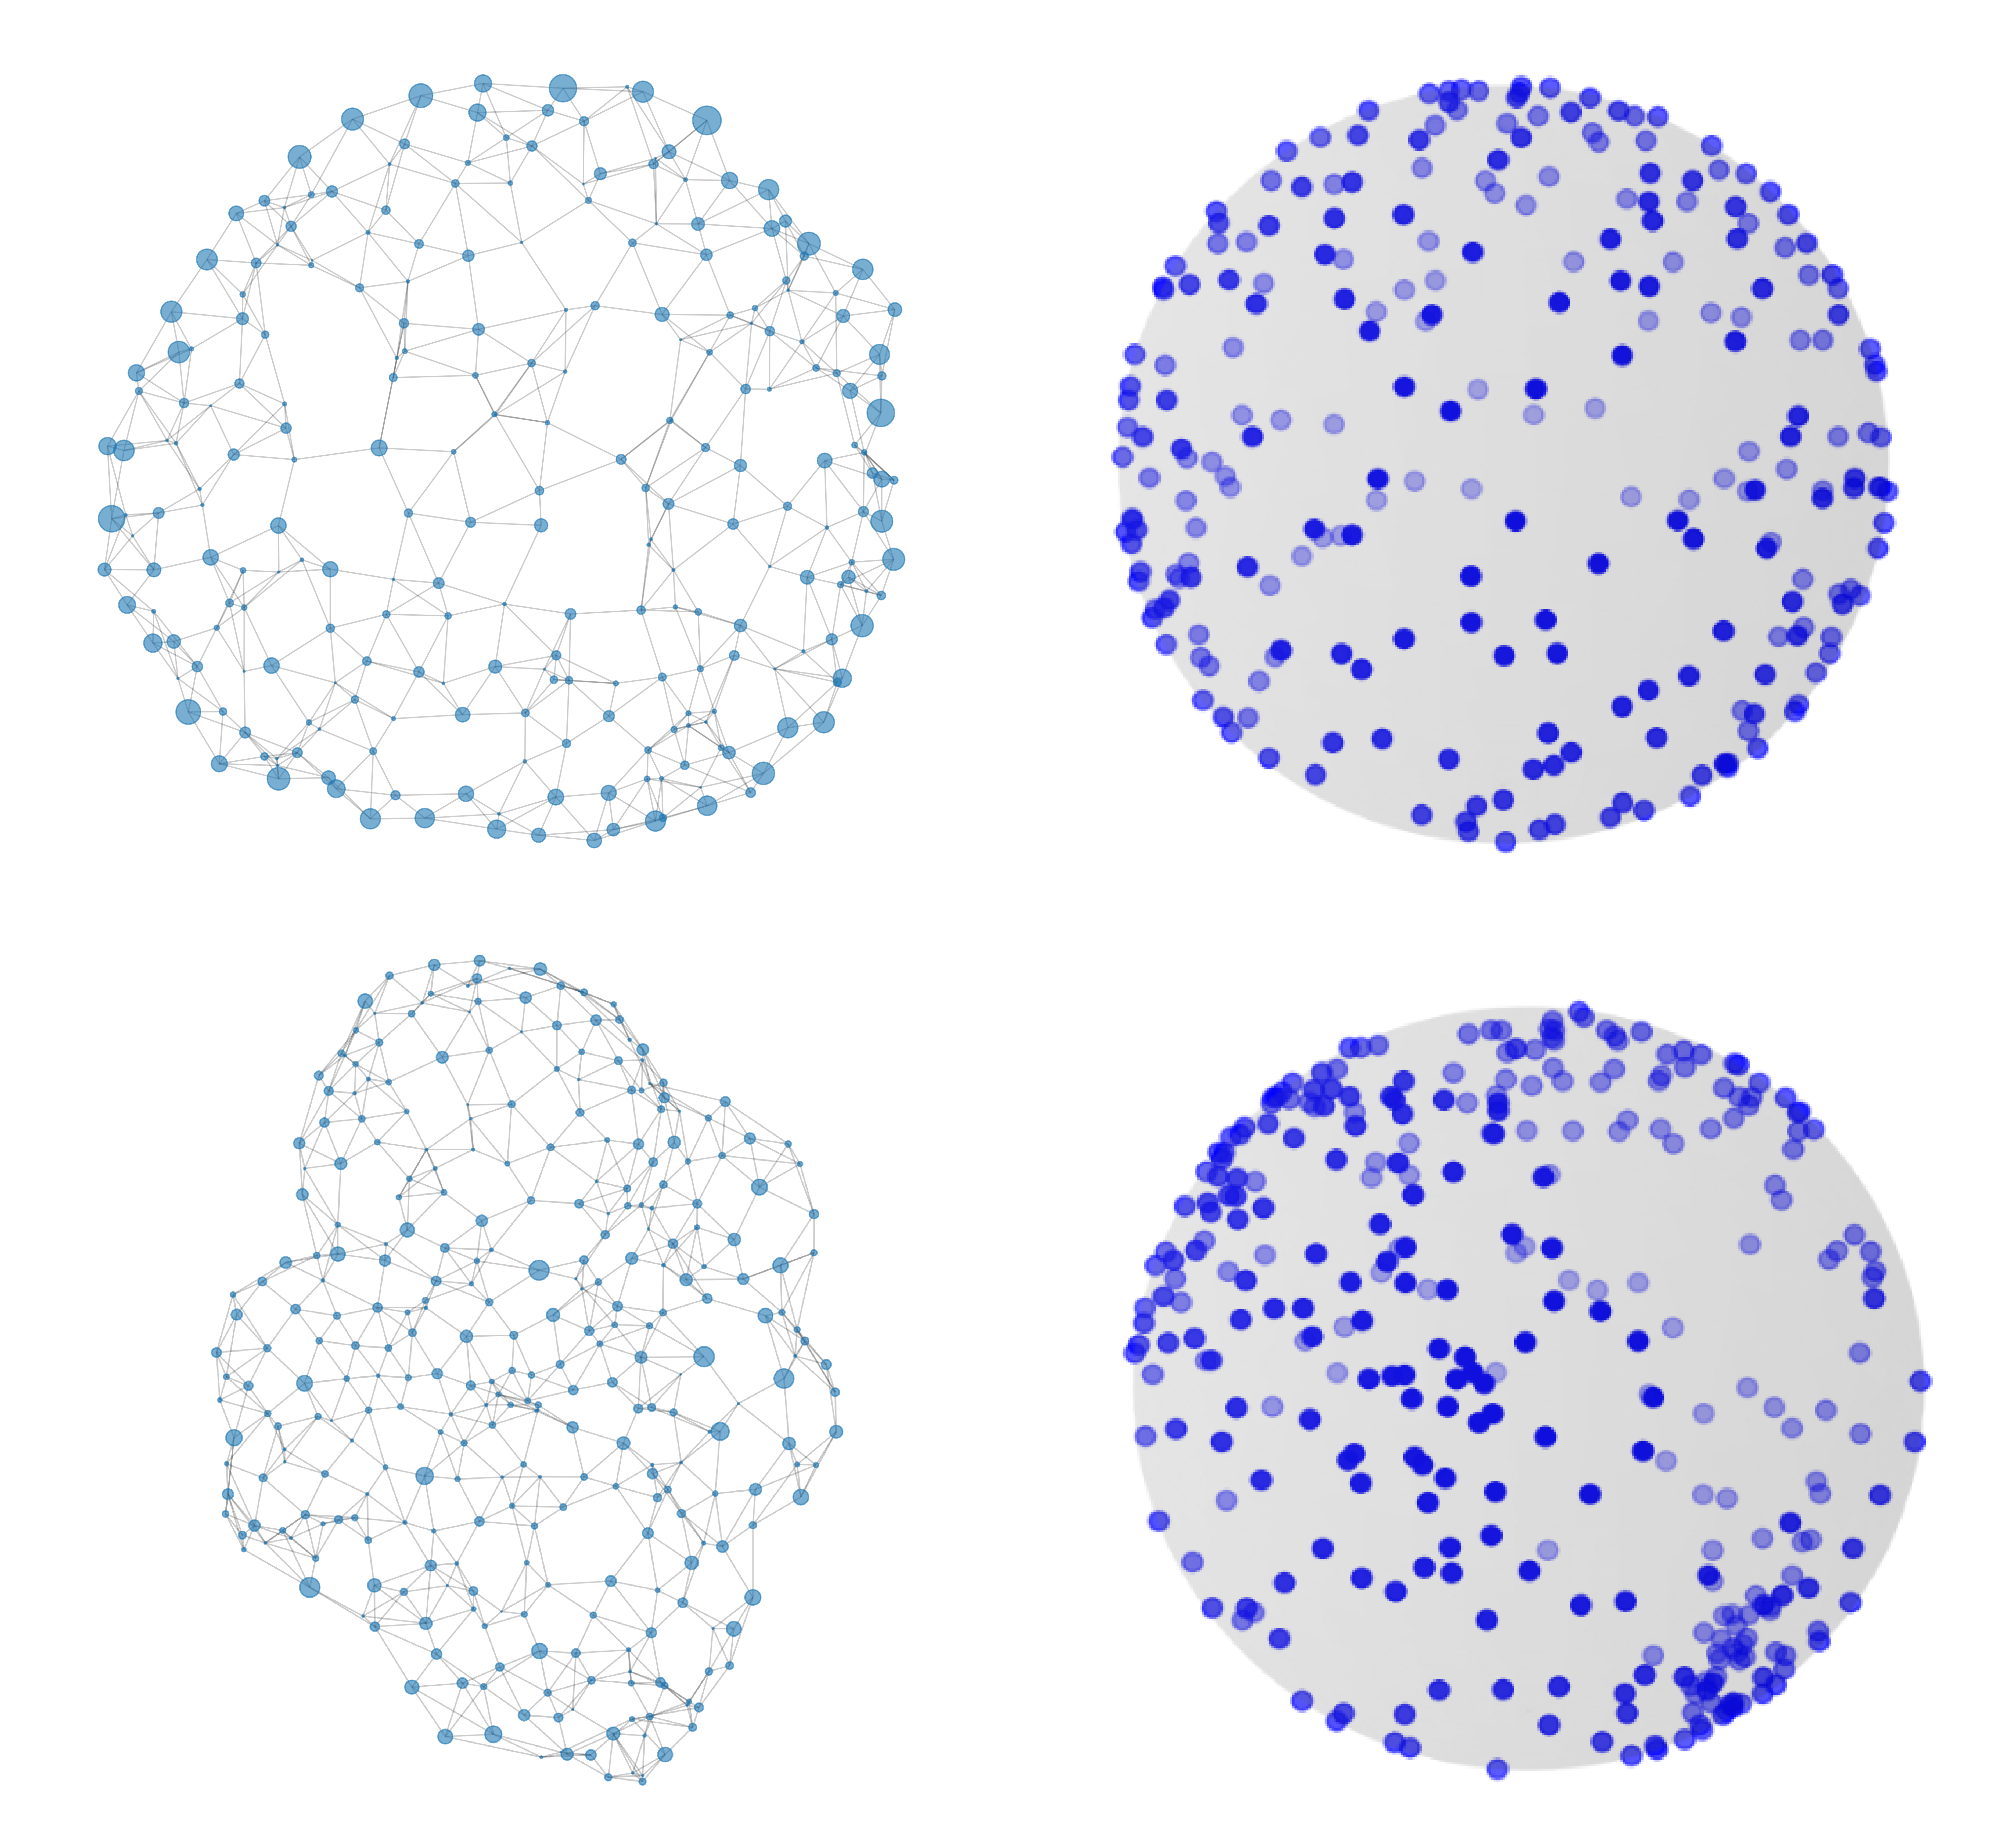
\includegraphics[width=0.95\textwidth]{../img/Modelisation.png}
    \caption{Distributions de points sur la sphère (à droite) et les organoïdes synthétiques étendus (à gauche) après transformation spatiale proportionnelle à la densité locale.}
    \label{fig:modelisation}
\end{figure}

Ce dataset synthétique sert deux objectifs majeurs : le pré-entraînement de nos architectures GNN pour acquérir des représentations robustes des patterns spatiaux cellulaires, et l'entraînement de régresseurs prédisant le coefficient de clustering à partir de la structure graphique — une tâche auxiliaire favorisant l'apprentissage de features géométriques pertinentes transférables à la classification de phénotypes réels.

\section{Architectures GNN implémentées}

\subsection{Architecture globale commune}

Toutes nos architectures partagent une structure modulaire :

\textbf{Schéma général :}
\begin{enumerate}
    \item \textbf{Input embedding} : $\mathbf{h}_i^{(0)} = \text{MLP}_{\text{in}}(\mathbf{f}_i)$, projette les features initiales dans l'espace latent
    \item \textbf{Couches de message passing} : $K$ couches transformant $\mathbf{h}_i^{(k-1)} \rightarrow \mathbf{h}_i^{(k)}$
    \item \textbf{Pooling global} : $\mathbf{h}_G = \text{POOL}(\{\mathbf{h}_i^{(K)}\})$, agrège au niveau du graphe
    \item \textbf{Classification head} : $\mathbf{y} = \text{MLP}_{\text{out}}(\mathbf{h}_G)$, prédit la distribution sur les classes
\end{enumerate}

\subsection{GCN baseline}

\textbf{Motivation :}
Référence simple et établie pour évaluer l'apport des architectures plus sophistiquées.

\textbf{Couche GCN :}
\[
\mathbf{h}_i^{(k+1)} = \sigma\left(\sum_{j \in \mathcal{N}(i) \cup \{i\}} \frac{1}{\sqrt{d_i d_j}} \mathbf{W}^{(k)}\mathbf{h}_j^{(k)}\right)
\]

\textbf{Hyperparamètres :}
\begin{itemize}
    \item Nombre de couches : 3
    \item Dimension cachée : 128
    \item Activation : ReLU
    \item Pooling : Global mean pooling
    \item Head : MLP 2 couches (256 → 128 → C classes)
\end{itemize}

\textbf{Nombre de paramètres :} ~250K

\subsection{GAT baseline}

\textbf{Motivation :}
Évaluer l'apport du mécanisme d'attention.

\textbf{Couche GAT multi-head :}
\[
\mathbf{h}_i^{(k+1)} = \|_{m=1}^M \sigma\left(\sum_{j \in \mathcal{N}(i)} \alpha_{ij}^m \mathbf{W}^{m,(k)}\mathbf{h}_j^{(k)}\right)
\]

\textbf{Hyperparamètres :}
\begin{itemize}
    \item Nombre de couches : 3
    \item Têtes d'attention : 4
    \item Dimension cachée : 128 (32 par tête)
    \item Dropout attention : 0.1
    \item Pooling : Global attention-weighted pooling
\end{itemize}

\textbf{Nombre de paramètres :} ~320K

\subsection{EGNN principal}

\textbf{Motivation :}
Architecture principale, exploite pleinement la géométrie 3D et garantit l'équivariance E(3).

\subsubsection{Couche EGNN}

\textbf{Messages :}
\[
\mathbf{m}_{ij} = \phi_e\left([\mathbf{h}_i \| \mathbf{h}_j \| \|\mathbf{x}_i - \mathbf{x}_j\|^2]\right)
\]

où $\phi_e$ est un MLP (embedding → 128 → 128 → message\_dim).

\textbf{Agrégation :}
\[
\mathbf{m}_i = \sum_{j \in \mathcal{N}(i)} \mathbf{m}_{ij}
\]

\textbf{Mise à jour coordinates :}
\[
\mathbf{x}_i' = \mathbf{x}_i + C \sum_{j \in \mathcal{N}(i)} (\mathbf{x}_i - \mathbf{x}_j) \cdot \phi_x(\mathbf{m}_{ij})
\]

où $\phi_x$ prédit un coefficient scalaire, $C = 1/|\mathcal{N}(i)|$ normalisation.

\textbf{Mise à jour features :}
\[
\mathbf{h}_i' = \phi_h([\mathbf{h}_i \| \mathbf{m}_i])
\]

où $\phi_h$ est un MLP.

\subsubsection{Hyper paramètres}

\begin{itemize}
    \item Nombre de couches : 5 (plus profond que les baselines car moins d'over-smoothing)
    \item Dimension cachée : 256
    \item Message dimension : 128
    \item Activation : SiLU (Swish)
    \item Dropout : 0.15
    \item Normalisation : Layer Norm après chaque couche
    \item Pooling : Mean + Max pooling concaténés
\end{itemize}

\textbf{Nombre de paramètres :} ~800K

\subsubsection{Adaptations spécifiques}

Nous proposons des modifications à l'EGNN standard :

\textbf{Attention géométrique :}
Pondération des messages par une fonction de distance :
\[
\mathbf{m}_{ij}' = \mathbf{m}_{ij} \cdot \exp(-d_{ij}^2 / 2\sigma^2)
\]

Les voisins proches contribuent plus que les voisins distants.

\textbf{Multi-scale aggregation :}
Agrégation à différents niveaux de voisinage (1-hop, 2-hop) :
\[
\mathbf{m}_i = \mathbf{m}_i^{(1)} \| \mathbf{m}_i^{(2)}
\]

Capture les patterns locaux et plus globaux simultanément.

\subsection{Variante : GNN hiérarchique}

Pour les très grands organoïdes, nous implémentons un pooling hiérarchique :

\textbf{Architecture :}
\begin{enumerate}
    \item EGNN couches 1-3 : message passing au niveau cellulaire
    \item Pooling : Regroupement de cellules en super-nœuds (TopK ou DiffPool)
    \item EGNN couches 4-5 : message passing au niveau super-nœuds
    \item Pooling global : Agrégation finale
\end{enumerate}

\textbf{Avantage :} Réduction de la complexité pour les organoïdes de plus de 1000 cellules.

\section{Entraînement et optimisation}

\subsection{Fonction de perte}

\subsubsection{Cross-entropy pour classification}

Pour la classification multi-classes, nous utilisons la cross-entropy :
\[
\mathcal{L}_{\text{CE}} = -\frac{1}{B}\sum_{b=1}^B \sum_{c=1}^C y_{bc} \log(\hat{y}_{bc})
\]

où $B$ est la taille du batch, $C$ le nombre de classes, $y_{bc}$ le label one-hot, $\hat{y}_{bc}$ la probabilité prédite (après softmax).

\subsubsection{Pondération pour déséquilibre de classes}

En cas de déséquilibre, nous utilisons une pondération :
\[
\mathcal{L}_{\text{weighted}} = -\frac{1}{B}\sum_{b=1}^B \sum_{c=1}^C w_c \cdot y_{bc} \log(\hat{y}_{bc})
\]

avec $w_c = \frac{N_{\text{total}}}{C \cdot N_c}$ (inverse fréquence).

\subsubsection{Régularisation}

\textbf{L2 weight decay :}
\[
\mathcal{L}_{\text{total}} = \mathcal{L}_{\text{CE}} + \lambda_{\text{reg}} \sum_{\ell} \|\mathbf{W}^{(\ell)}\|_F^2
\]

avec $\lambda_{\text{reg}} = 10^{-5}$.

\textbf{Dropout :}
Nous appliquons un dropout (taux 0.15) sur les features de nœuds entre couches, ainsi que sur les arêtes.

\subsection{Optimisation}

\subsubsection{Algorithme d'optimisation}

\textbf{AdamW :}
Nous utilisons AdamW (Adam avec weight decay découplé) :
\begin{itemize}
    \item Learning rate initial : $10^{-3}$
    \item $\beta_1 = 0.9$, $\beta_2 = 0.999$
    \item Weight decay : $10^{-5}$
    \item Gradient clipping : norm max 1.0
\end{itemize}

\subsubsection{Learning rate scheduling}

\textbf{ReduceLROnPlateau :}
Réduction du learning rate si la métrique de validation stagne :
\begin{itemize}
    \item Facteur : 0.5
    \item Patience : 10 époques
    \item LR minimum : $10^{-6}$
\end{itemize}

\subsubsection{Early stopping}

Nous arrêtons l'entraînement si la métrique de validation ne s'améliore pas pendant 20 époques consécutives et restaurons les poids de la meilleure époque.

\subsection{Stratégies d'entraînement}

\subsubsection{Entraînement sur synthétiques}

\textbf{Phase 1 : Pré-entraînement}
\begin{itemize}
    \item Dataset : 70~000 organoïdes synthétiques (train)
    \item Batch size : 32 graphes
    \item Époques : 200
    \item Durée : ~48 heures (GPU NVIDIA RTX 3080)
\end{itemize}

\subsubsection{Fine-tuning sur réels}

\textbf{Phase 2 : Adaptation au réel}
\begin{itemize}
    \item Initialisation : Poids pré-entraînés (sauf classification head, réinitialisée)
    \item Dataset : N organoïdes réels annotés (typiquement N = 500)
    \item Learning rate réduit : $10^{-4}$ (fine-tuning)
    \item Époques : 100
    \item Régularisation accrue : dropout 0.2, weight decay $10^{-4}$
\end{itemize}

\subsubsection{Entraînement from scratch sur réels}

\textbf{Baseline sans pré-entraînement :}
Pour comparaison, nous entraînons également des modèles directement sur les 500 organoïdes réels annotés depuis une initialisation aléatoire.

\subsection{Validation croisée}

\subsubsection{Stratégie}

\textbf{5-fold stratified cross-validation :}
\begin{enumerate}
    \item Partitionner le dataset en 5 folds stratifiés (distribution de classes préservée)
    \item Pour chaque fold :
    \begin{enumerate}
        \item Entraîner sur 4 folds
        \item Valider sur 1 fold
    \end{enumerate}
    \item Agréger les résultats (moyenne et écart-type des métriques)
\end{enumerate}

\textbf{Nested cross-validation :}
Pour éviter tout biais lors du choix des hyperparamètres, nous appliquons une nested cross-validation : la boucle extérieure (5 folds) sert à estimer la performance, tandis que la boucle intérieure (3 folds) optimise les hyperparamètres uniquement sur les données d’entraînement.

\subsubsection{Importance de la stratification}

La stratification assure que chaque fold contient une proportion représentative de chaque classe, crucial avec des datasets de petite taille et des classes potentiellement déséquilibrées.

\subsection{Recherche d'hyperparamètres}

\subsubsection{Espace de recherche}

Hyperparamètres explorés :
\begin{itemize}
    \item Nombre de couches : \{3, 4, 5, 6\}
    \item Dimension des couches cachées : \{64, 128, 256, 512\}
    \item Learning rate : \{$10^{-4}$, $5 \times 10^{-4}$, $10^{-3}$, $5 \times 10^{-3}$\}
    \item Dropout : \{0.0, 0.1, 0.15, 0.2, 0.3\}
    \item Batch size : \{16, 32, 64\}
    \item K (connectivité K-NN) : \{5, 8, 10, 12, 15\}
\end{itemize}

\subsubsection{Stratégie de recherche}

\textbf{Random search :}
Plutôt que la grid search (combinatoire, coûteuse), nous échantillonnons aléatoirement 100 configurations et entraînons chacune pour 50 époques.

\textbf{Critère de sélection :}
Accuracy moyenne sur le validation set du inner cross-validation loop.

\subsubsection{Résultats}

\textbf{Configuration optimale trouvée :}
\begin{itemize}
    \item Couches : 5
    \item Dimension : 256
    \item LR : $10^{-3}$
    \item Dropout : 0.15
    \item Batch : 32
    \item K : 10
\end{itemize}

\textbf{Sensibilité :}
La dimension cachée et le nombre de couches sont les plus impactants. Le learning rate et le dropout ont un effet modéré dans les plages explorées.

\section{Récapitulatif méthodologique}

Ce chapitre a décrit en détail chaque composante de notre pipeline innovant pour l'analyse automatisée d'organoïdes 3D via Graph Neural Networks.

\textbf{Prétraitement et segmentation} : Le pipeline débute par un prétraitement robuste (normalisation d'intensité par percentiles, débruitage) suivi d'une segmentation state-of-the-art via Faster Cellpose

\textbf{Données réelles et tâches} : Notre dataset collaboratif comprend 1311 échantillons imagés (2272 organoïdes extraits), dont nous avons sélectionné ~500 organoïdes bien différenciés (~250 par classe) pour l'apprentissage supervisé. Les phénotypes étudiés sont : choux-fleurs (agrégation spatiale forte) et cystiques (répartition homogène). Nous adressons trois tâches complémentaires : classification binaire choux-fleurs vs cystiques (tâche principale), régression du coefficient de clustering sur synthétiques (pré-entraînement), et régression de la déformation morphologique sur réels (quantification fine).

\textbf{Génération synthétique} : Contribution majeure, nos ~100~000 organoïdes synthétiques sont générés via processus ponctuels (Poisson homogène et Matérn cluster) formant un continuum contrôlé de patterns spatiaux. La génération initiale sur la sphère permet la validation statistique rigoureuse (fonctions de Ripley, tests KS) ; le dataset GNN final subit ensuite une transformation spatiale étendant les coordonnées au-delà de la sphère proportionnellement à la densité locale, simulant les protubérances "chou-fleur" tout en préservant les aires cellulaires. Ces synthétiques servent au pré-entraînement et à l'apprentissage de représentations géométriques transférables.

\textbf{Construction de graphes} : Extraction de 4 features par cellule (coordonnées 3D, volume), puis construction via stratégie K-NN hybride (k=10) équilibrant connectivité, signification biologique et efficacité computationnelle.

\textbf{Architectures et entraînement} : Nous comparons plusieurs architectures GNN : GAT (Graph Attention Network), DeepSets, EGNN équivariant, et GCN comme baseline. Stratégie d'entraînement en deux phases : pré-entraînement sur synthétiques (régression clustering) puis fine-tuning sur réels (classification/régression), avec validation croisée 5-fold et recherche d'hyperparamètres systématique.

Le Chapitre 5 présentera les résultats expérimentaux obtenus avec cette méthodologie, validant empiriquement les choix effectués et quantifiant les performances sur les tâches de classification et de régression.
